\documentclass[10pt,journal,epsfig,onecolumn]{IEEEtran}
\usepackage{blindtext}
\usepackage{graphicx}
\usepackage{amsmath}
\usepackage{amssymb}
\usepackage{arydshln}
\usepackage{color}
\usepackage{algorithm}
\usepackage{algorithmic}
\usepackage{amsthm}
\usepackage{color}
\usepackage{multirow}
\usepackage{subfigure}


\newtheorem{definition}{Definition}
\newtheorem{remark}{Remark}
\newtheorem{assumption}{Assumption}
\newtheorem{theorem}{Theorem}
\newtheorem{proposition}{Proposition}
\newtheorem{lemma}{Lemma}
\newtheorem{corollary}{Corollary}

\newcommand{\tabincell}[2]{\begin{tabular}{@{}#1@{}}#2\end{tabular}}

%%%%%������: ѡ���������


\begin{document}
%
% paper title
% can use linebreaks \\ within to get better formatting as desired
\title{A Dynamic Neural Network Approach for Solving Nonlinear Inequalities Defined on A Graph and Its Application to Distributed, Routing-free, Range-free Localization of WSNs}


\author{Shuai~Li and Feng Qin%,~\IEEEmembership{Member,~IEEE,}% <-this % stops a space
\thanks{S. Li is with department of Electrical and Computer Engineering, Stevens Institute of Technology, Hoboken, NJ 07030, USA. F. Qin is with the School of Computer Science, Anhui University of Technology, Ma'anshan, Anhui, China. Emails: lshuai@stevens.edu (S. Li), and fqin@ahut.edu.cn (F. Qin).}
}

%%%%1.������Ŀ
\maketitle
\begin{abstract}
In this paper, we are concerned with the problem of finding a feasible solution to a class of nonlinear inequalities defined on a graph. A recurrent neural network is proposed to tackle this problem. The convergence of the neural network and the solution feasibility to the defined problem are both theoretically proven. The proposed neural network features a parallel computing mechanism and a distributed topology isomorphic to the corresponding graph. Thus it is suitable for distributed real-time computation. The proposed neural network is applied to  range-free localization of wireless sensor networks (WSNs). The analog circuit implementation of the neural network for such an application is also explored. Simulations demonstrate the effectiveness of the proposed method.
\end{abstract}








\begin{IEEEkeywords}
Recurrent neural network, wireless sensor networks, range-free localization, distributed estimation, routing-free localization.
\end{IEEEkeywords}
\IEEEpeerreviewmaketitle




\section{Introduction}
Large scale networks widely exist in natural or man-made systems. Typical examples include metabolic networks \cite{jeong2000}, power networks \cite{Buldyrev2009}, wireless sensor networks (WSNs) \cite{Akyildiz02}, robot networks \cite{Cao97}, etc. Many problems associated with large scale networks, are emerging and receiving intensive studies. For example, the problem of predicting protein folding pathways can be defined as an global minimization problem defined on a graph formed by amino acid sequence \cite{Zaki2004}; the cooperative control of robot networks can be modeled as a dynamic programming problem defined on a graph constructed by robot interactions \cite{DistCtrlRobotNetw}. Particularly, there is a class of widely existing  problems associated with a large scale network, which can be described by a set of nonlinear inequalities relevant to the interactions between agents. For instance, the communication connectivity  maintenance of a robot network is concerned with forming a topological structure, on which the distance  between neighbor robots does not exceed the limit of communication range \cite{Reich2011}; the range-free localization of WSNs is concerned finding an estimation of sensor node positions, which does not violate the proximity topology constraints \cite{Kulaib}. In this paper, we formulate this class of problems in an unified framework as nonlinear inequalities defined on a graph. For problems defined on a graph with a huge number of agents involved,  traditional centralized methods are challenged for scenarios with no powerful central computers. In contrast, distributed methods, which allocate  the whole complicated task to every agents on the graph and solve the problem cooperatively, demonstrate  great attractions.

In recent years, recurrent neural networks have received considerable studies in signal processing \cite{Skowronski}, pattern classification \cite{Niranjan,Husken}, robotics \cite{Ogata}, optimization \cite{Smith}, etc. Particularly, after the invention of the Hopfield neural network \cite{Hopfield_1984}, which was originally designed for online optimization, recurrent neural networks, resulting from its parallelism and online solving capability,  are becoming more and more popular in online optimization \cite{zhangglobal}. In this paper, we design a recurrent neural network to tackle the formulated nonlinear inequality problem defined on a graph in real time and apply the neural network model to range-free localization of WSNs.




To a constrained optimization problem, early works on recurrent neural networks \cite{Hopfield_1984,Kennedy783} often design a recurrent neural network evolving along the gradient descent direction of an augmented energy function formed by introducing a constraint-related penalty term into the objective function. However, the solution of the neural network often has a small deviation from the optimal one due to the compromise between the cost function and the constraints. To remedy this, \cite{Zhang2002271,Xia122004} study the problem in the dual space and use a projection function to represent inequality constraints. For the case with linear inequality constraints, it is proven in theory that this type of methods are able to converge to the optimal solution. The results are latter applied to various applications, such as kinematic control of redundant manipulators \cite{Zhang03},  k-winner-take-all (k-WTA) problem solving \cite{Liu06}, $L_1$ norm estimation \cite{Xia_2009},  to exploit the real-time processing capability of the neural networks. Successive works \cite{Xia22008,Jiang201297,springerlinkliu} in this field extend the results to the cases with nonlinear constraints with guaranteed convergence of the recurrent neural network. Although great success has been gained in the field of using recurrent neural networks to solve constrained optimization, difficulties are encountered when  using recurrent neural networks to solve  nonlinear inequalities defined on a large scale graph as the recurrent neural network approach is essentially a centralize method and is not scalable to a large networked systems. By taking advantage of the local connection between nodes on a graph, a distributed recurrent neural network, whose topology is isomorphic to the graph topology, is elaborately designed to solve nonlinear inequalities defined on the graph in a decentralized fashion.

A prominent feature of the proposed neural network to solve nonlinear inequalities defined on a graph is that its topology is isomorphic to the graph topology, i.e., each neuron in the neural network corresponds to a node on the graph and the neural connections corresponds to edges on the graph, which is in contrast to the conventional neural networks with connections between all pairs of neurons. For applications, this topological feature enables distributed computation, which is often necessary for a scalable large scale network.

The remainder of this paper is organized as follows. In Section \ref{formulateproblem}, we present the neural network model for solving the nonlinear inequality problem defined on a graph. In Section \ref{theorey}, the convergence of the neural network is analyzed and it is proven to be  convergent to a feasible solution of the problem. In Section \ref{myla}, the neural network model is applied to solve range-free localization of WSNs. Its hardware implementation is explored in Section \ref{hardwareee}. In Section \ref{simmm}, simulation examples are given to demonstrate the effectiveness of our method. Section \ref{cons} concludes this paper.


\section{Model Description}\label{formulateproblem}
In this section, we are concerned with inequalities defined on a graph  $\mathcal{G}(\mathbb{V}, \mathbb{E})$ (where $\mathbb{V}$ and $\mathbb{E}$ denote the vertex set and the edge set, respectively) with the following expression:
\begin{eqnarray}\label{problem}
f_{ij}(x_i,x_j) \leq 0 \quad\text{for}\, j\in \mathbb{N}(i) \bigcup \{i\}, \forall i\in \mathbb{V}
\end{eqnarray}
where $\mathbb{N}(i)$ denotes the neighbor set of vertex $i$, which is defined as $\mathbb{N}(i)=\{j\in \mathbb{V}| \{i, j\}\in \mathbb{E}\}$. $x_i\in \mathbb{R}^m$ is the state variable associated with vertex $i$. $f_{ij}(x_i,x_j)\in\mathbb{R}$ is a nonlinear convex  function with respect to $x_i$ and $x_j$.

Note that there is no explicit objective function but inequality constraints  in problem (\ref{problem}).  Mostly, the solution to this problem is not unique. In some applications, such as range-free localization of WSNs \cite{Doherty,he2003} (as detailed in Section \ref{myla}) and communication connectivity maintenance in robot networks \cite{Reich2011,Hsieh2008}, researchers are more concerned with finding a feasible solution in real time  instead of finding all the feasible solutions. Based on this consideration, we explore finding a feasible solution to problem (\ref{problem}) in real time via a recurrent dual neural network.

Problem (\ref{problem}) is equivalent to the following normal optimization problem by augmenting the original problem with a virtual objective function,
\begin{eqnarray}\label{problem1}
\leftline{$\text{minimize} \quad\, J =0$} \nonumber\\
\leftline{$\text{subject to} \quad f_{ij}(x_i,x_j) \leq 0 \quad\text{for}\, j\in \mathbb{N}(i) \bigcup \{i\}, \forall i\in \mathbb{V}$}
\end{eqnarray}
where $J$ is the virtual objective function. According to Karash-Kuhn-Tucker (KKT) conditions \cite{Boyd04}, the solution to problem (\ref{problem1}) satisfies,
\begin{subequations}\label{kkt}
\begin{eqnarray}
&\lambda_{ii}\frac{\partial f_{ii}(x_i, x_i)}{\partial x_i}+\sum_{j\in\mathbb{N}(i)}\big(\lambda_{ij}\frac{\partial f_{ij}(x_i, x_j)}{\partial x_i}+\lambda_{ji}\frac{\partial f_{ji}(x_j, x_i)}{\partial x_i}\big)=0 \,\,\forall i\in \mathbb{V}\label{kkt1}\\
&f_{ij}(x_i,x_j)\left\{
\begin{array}{cc}
=0  & \quad(\lambda_{ij}>0)\\
<0 &  \quad(\lambda_{ij}=0)
\end{array}
\right. \quad\text{for}\, j\in \mathbb{N}(i) \bigcup \{i\}, \forall i\in \mathbb{V}\label{kkt22}
\end{eqnarray}
\end{subequations}
where $\lambda_{ij}\in\mathbb{R}$, $\lambda_{ji}\in\mathbb{R}$ and $\lambda_{ii}\in\mathbb{R}$ are all dual variables. Note that (\ref{kkt22}) can be simplified into the following form,
\begin{eqnarray}\label{newkkt3}
g\big(f_{ij}(x_i, x_j)+\lambda_{ij}\big)=\lambda_{ij}\quad\text{for}\, j\in \mathbb{N}(i) \bigcup \{i\}, \forall i\in \mathbb{V}
\end{eqnarray}
with the function $g(u)=[g_1(u_1), g_2(u_2), ..., g_k(u_k)]^T$ for $u=[u_1, u_2, ..., u_k]^T$ defined as follows for $i=1, 2, ..., k$,
\begin{eqnarray}\label{satur}
g_i(u_i)=\left\{
\begin{aligned}
&u_i&    \,  \, &\text{if} \,  \, u_i > 0&\\
&0&   \,  \,  &\text{if}  \, \, u_i\leq 0&
\end{aligned}
\right.
\end{eqnarray}
%Substituting (\ref{newkkt3}) into (\ref{kkt1}), we get,
%\begin{eqnarray}\label{revise}
%g\big(f_{ii}(x_i, x_i)+\lambda_{ii}\big)\frac{\partial f_{ii}(x_i, x_i)}{\partial x_i}+\sum_{j\in\mathbb{N}(i)}\bigg(g\big(f_{ij}(x_i, x_j)+\lambda_{ij}\big)\frac{\partial f_{ij}(x_i, x_j)}{\partial x_i}\nonumber\\
%+g\big(f_{ji}(x_j, x_i)+\lambda_{ji}\big)\frac{\partial f_{ji}(x_j, x_i)}{\partial x_i}\bigg)=0 \,\,\forall i\in \mathbb{V}
%\end{eqnarray}
Up to now, the original inequality problem (\ref{problem}) is equivalently transformed to nonlinear equations consisting of (\ref{kkt1}) and (\ref{newkkt3}). We use a recurrent neural network to solve the variables in (\ref{kkt1}) and (\ref{newkkt3}) as follows:
\begin{eqnarray}\label{nnmodel}
\dot{x}_i&=&-\epsilon \bigg(\lambda_{ii}\frac{\partial f_{ii}(x_i, x_i)}{\partial x_i}+\sum_{j\in\mathbb{N}(i)}\big(\lambda_{ij}\frac{\partial f_{ij}(x_i, x_j)}{\partial x_i}+\lambda_{ji}\frac{\partial f_{ji}(x_j, x_i)}{\partial x_i}\big)\bigg) \,\,\forall i\in \mathbb{V}\nonumber\\
\dot{\lambda}_{ij}&=&\epsilon g\big(f_{ij}(x_i, x_j)+\lambda_{ij}\big)-\epsilon {\lambda}_{ij}\quad\text{for}\, j\in \mathbb{N}(i) \bigcup \{i\}, \forall i\in \mathbb{V}
\end{eqnarray}
where $\epsilon>0$ is a scaling factor, the function $g(\cdot)$ is defined in (\ref{satur}), $\lambda_{ij}\in\mathbb{R}$, $\lambda_{ii}\in\mathbb{R}$ and $\lambda_{ji}\in\mathbb{R}$ are dual variables associated with the edge $\{i, j\}\in\mathbb{E}$, the vertex $i$, and the edge $\{j, i\}\in\mathbb{E}$, respectively. About the distributiveness of the proposed neural network model (\ref{nnmodel}), we have the following remark.%About this neural network model (\ref{nnmodel}), we have the following remark,
%\begin{remark}\label{remakr1}
%Actually, the equation set composed of (\ref{kkt1}) and (\ref{newkkt3}) is also equivalent to the original inequality problem (\ref{problem}). A straightforward thinking is to use the following neural network:
%\begin{eqnarray}\label{nnmodel2}
%\dot{x}_i&=&-2\epsilon \lambda_{ii}\frac{\partial f_{ii}(x_i, x_i)}{\partial x_i}+\big(\sum_{j\in\mathbb{N}(i)}\lambda_{ij}\frac{\partial f_{ij}(x_i, x_j)}{\partial x_i}+\lambda_{ji}\frac{\partial f_{ji}(x_j, x_i)}{\partial x_i}\big) \,\,\forall i\in \mathbb{V}\nonumber\\
%\dot{\lambda}_{ij}&=&\epsilon g\big(f_{ij}(x_i, x_j)+\lambda_{ij}\big)-\epsilon {\lambda}_{ij}\quad\text{for}\, j\in \mathbb{N}(i) \bigcup \{i\}, \forall i\in \mathbb{V}
%\end{eqnarray}
%However, this neural network may diverge if not properly initialized. In contrast, the stability of the neural network (\ref{nnmodel}) can be strictly proven and the result always converges to an equilibrium under any initializations as proven in Section \ref{theorey}. That is why we use the neural network (\ref{nnmodel}) instead of (\ref{nnmodel2}).
%\end{remark}



In the dynamic equation (\ref{nnmodel}), the update of $x_i$, which is associated with the vertex $i$,   requires information on the value of $x_i$ itself,  the value of $x_{j}$ for $j\in\mathbb{N}(i)$, which is associated with $i$'s neighbor vertex $j$, the value of $\lambda_{ii}$ associated with the vertex $i$, the value of $\lambda_{ij}$ associated with the edge  $\{i, j\}\in\mathbb{E}$ and the value of $\lambda_{ji}$ associated with the edge  $\{j, i\}\in\mathbb{E}$. All the above required information comes either from the vertex $i$ itself or from its neighbor vertices or the edges in between. On the other hand, for the update of $\lambda_{ij}$, which is associated with the edge $\{i, j\}\in\mathbb{E}$, the required information includes  the value of $\lambda_{ij}$ itself, the value of $x_i$ and the value of $x_j$, which are associated with the two vertices forming the edge $\{i, j\}$. Clearly, all the required information for the update of $\lambda_{ij}$ is available in the neighborhood. In this sense, the neural network (\ref{nnmodel}) has an isomorphic topology to  the graph $\mathcal{G}(\mathbb{V}, \mathbb{E})$.

\begin{remark}\label{distributedmodel}
The connection topology of the neural network model (\ref{nnmodel}) is isomorphic to the graph $\mathcal{G}(\mathbb{V}, \mathbb{E})$, on which the problem (\ref{problem}) is defined. This property enables us to implement  the neural network in a distributed fashion by assigning the state variables $x_i$, $\lambda_{ii}$ and $\lambda_{ij}$ for all $j\in\mathbb{N}(i)$ to the vertex $i$. In this way, for the dynamic evolution of the neural network (\ref{nnmodel}), communications only happen between neighbor vertices and neither routing nor cross-hop communication is required, which thoroughly reduces the communication burden especially for the case with a large number of vertices.
\end{remark}





For the convenience of analysis, the neural network dynamic (\ref{nnmodel}) can be equivalently written into a compact form,
\begin{eqnarray}\label{nnmodelvector}
\dot{x}&=&-\epsilon\big(\nabla^T \bar{F}(x)\big)\bar{\Lambda}\nonumber\\
\dot{\bar{\Lambda}}&=&\epsilon \bigg(g\big(\bar{F}(x)+\bar{\Lambda}\big)- {\bar{\Lambda}}\bigg)
\end{eqnarray}
where $x$ is a $mn$ dimensional vector with $n=|\mathbb{V}|$ denoting the number of vertices on the graph, $m$ denoting the dimension of $x_i$ for $i\in\mathbb{V}$ and  $x=[x_1^T, x_2^T, ..., x_n^T]^T$, $F(x)\in\mathbb{R}^{n\times n}$ is a matrix function of $x$ with the $ij$th entry defined as follows:
\begin{eqnarray}
F_{ij}(x)=\left\{
\begin{aligned}
f_{ij}(x_i, x_j) & \quad\text{for}\,\, i\in\mathbb{V}, j\in\mathbb{V} \,\text{and}\, j\in\mathbb{N}(i)\\
0 & \quad\text{for} \,\, i\in\mathbb{V}, j\in\mathbb{V} \,\text{and}\, j \notin \mathbb{N}(i)
\end{aligned}
\right.
\end{eqnarray}
Similarly, $\Lambda\in\mathbb{R}^{n\times n}$ is defined as:
\begin{eqnarray}
\Lambda_{ij}=\left\{
\begin{aligned}
\lambda_{ij} & \quad\text{for}\,\, i\in\mathbb{V}, j\in\mathbb{V} \,\text{and}\, j\in\mathbb{N}(i)\\
\mu_{ij} & \quad\text{for} \,\, i\in\mathbb{V}, j\in\mathbb{V} \,\text{and}\, j \notin \mathbb{N}(i)
\end{aligned}
\right.
\end{eqnarray}
where $\mu_{ij}\in\mathbb{R}$ and is always initialized to be zero, i.e., $\mu_{ij}(0)=0$. In (\ref{nnmodelvector}), $\bar{F}(x)$ is defined to be  a $n^2$ dimensional vector by stacking the columns of $F(x)$ into a single column vector and $\bar{\Lambda}$ is so defined by stacking the columns of $\Lambda$ into a single column vector.

Note that $\mu_{ij}$ for $i\in\mathbb{V}, j\in\mathbb{V} \,\text{and}\, j \notin \mathbb{N}(i)$ is a redundant variable designed for the compactness of (\ref{nnmodelvector}). Since $F_{ij}(x)$ is zero  and $\mu_{ij}$ is initialized to be zero for $j \notin \mathbb{N}(i)$, $\mu_{ij}$ will be zero all the time after initialization according to the dynamics of (\ref{nnmodelvector}). With this in mind, the equivalence of the dynamic of the neural network  (\ref{nnmodel}) and its compact form (\ref{nnmodelvector}) can be verified by expanding the right-hand side of (\ref{nnmodelvector}) in entrywise and comparing it with the right-handside of (\ref{nnmodel}).







\section{Theoretical Results}\label{theorey}
In this section, we study  the convergence of the neural network (\ref{nnmodel}) and the solution feasibility to the original problem (\ref{problem}). Before starting up, we first state some useful conclusions for the proof.





\begin{lemma}\label{lemma1}
 The equilibrium point ${x_{i}^*, \lambda_{ij}^*}$ for all $i\in\mathbb{V}$, $j\in\mathbb{N}(i)\bigcup{i}$ of the recurrent neural network (\ref{nnmodel}) is a  solution to the problem (\ref{problem}).
\end{lemma}
\begin{proof}
The equilibrium point satisfies:
\begin{subequations}\label{equ}
\begin{eqnarray}
0&=&\lambda_{ii}^*\frac{\partial f_{ii}(x_i^*, x_i^*)}{\partial x_i}+\sum_{j\in\mathbb{N}(i)}\big(\lambda_{ij}^*\frac{\partial f_{ij}(x_i^*, x_j^*)}{\partial x_i}+\lambda_{ji}^*\frac{\partial f_{ji}(x_j^*, x_i^*)}{\partial x_i}\big) \,\,\forall i\in \mathbb{V}\label{equ1}\\
0&=& g\big(f_{ij}(x_i^*, x_j^*)+\lambda_{ij}^*\big)- {\lambda}_{ij}^*\quad\text{for}\, j\in \mathbb{N}(i) \bigcup \{i\}, \forall i\in \mathbb{V}\label{equ2}
\end{eqnarray}
\end{subequations}
With the definition of $g(\cdot)$ in (\ref{satur}), (\ref{equ2}) is equivalent to the following,
\begin{eqnarray}\label{sat1}
f_{ij}(x_i^*,x_j^*)\left\{
\begin{array}{cc}
=0  & \quad(\lambda_{ij}^*>0)\\
<0 &  \quad(\lambda_{ij}^*=0)
\end{array}
\right. \quad\text{for}\, j\in \mathbb{N}(i) \bigcup \{i\}, \forall i\in \mathbb{V}\label{kkt2}
\end{eqnarray}
(\ref{sat1}) and (\ref{equ1}) together form the KKT condition for problem (\ref{problem1}). As the function $J$ and the constraint $f_{ij}(x_i, x_j)\leq 0$ for $j\in\mathbb{N}(i)\bigcup\{i\}$, $i\in\mathbb{V}$ are convex, the KKT condition is necessary and sufficient  for problem (\ref{problem1}) and the equilibrium point ${x_{i}^*, \lambda_{ij}^*}$ for all $i\in\mathbb{V}$, $j\in\mathbb{N}(i)\bigcup{i}$ is an optimal solution to the problem. Further, resulting from the equivalence of problem (\ref{problem}) and problem (\ref{problem1}), we conclude that the equilibrium point ${x_{i}^*, \lambda_{ij}^*}$ for all $i\in\mathbb{V}$, $j\in\mathbb{N}(i)\bigcup{i}$ indeed satisfies problem (\ref{problem}). This completes the proof.
\end{proof}
%
%\begin{proposition}\label{proposition2}
% The equilibrium point ${x_{i}^*, \lambda_{ij}^*}$ for all $i\in\mathbb{V}$, $j\in\mathbb{N}(i)\bigcup{i}$ of the recurrent neural network (\ref{nnmodel}) satisfies the followings:
%\begin{subequations}\label{eqn}
%\begin{eqnarray}
%0&=&\lambda_{ii}^*\frac{\partial f_{ii}(x_i^*, x_i^*)}{\partial x_i}+\sum_{j\in\mathbb{N}(i)}\big(\lambda_{ij}^*\frac{\partial f_{ij}(x_i^*, x_j^*)}{\partial x_i}+\lambda_{ji}^*\frac{\partial f_{ji}(x_j^*, x_i^*)}{\partial x_i}\big) \,\,\forall i\in \mathbb{V}\label{equ11}\\
%0&=& g\big(f_{ij}(x_i^*, x_j^*)+\lambda_{ij}^*\big)- {\lambda}_{ij}^*\quad\text{for}\, j\in \mathbb{N}(i) \bigcup \{i\}, \forall i\in \mathbb{V}\label{equ22}\\
%0&\geq& f_{ij}(x_i^*, x_j^*)\quad\text{for}\, j\in \mathbb{N}(i) \bigcup \{i\}, \forall i\in \mathbb{V}\label{equ3}\\
%0&\leq&\lambda_{ij}^*\quad\text{for}\, j\in \mathbb{N}(i) \bigcup \{i\}, \forall i\in \mathbb{V}\label{equ4}\\
%0&\geq&\sum_{i\in\mathbb{V}}\sum_{j\in\mathbb{N}(i)\bigcup\{i\}}\big(\lambda_{ij}^* f_{ij}(x_i^*, x_j^*)\big)\quad \forall i\in \mathbb{V}\label{equ5}
%\end{eqnarray}
%\end{subequations}
%\end{proposition}
%In Proposition \ref{proposition2}, equations  (\ref{equ11}) and (\ref{equ22}) are direct results by solving the equilibrium point of the ordinary differential equation in (\ref{nnmodel}).  According to Lemma \ref{lemma1}, the equilibrium point is also a solution to the problem (\ref{problem}), so inequality (\ref{equ3}) holds. Inequality (\ref{equ4}) is obtained by noticing that $g(\cdot)\geq 0$ always holds according to the definition of $g(\cdot)$ in (\ref{satur})  and applying this observation to (\ref{equ22}). (\ref{equ5}) is a direct conclusion from (\ref{equ3}) and (\ref{equ4}).
%
%
%
%\begin{proposition}\label{proposition1}
%The function $g(\cdot)$ defined in (\ref{satur}) has the following property:
%\begin{eqnarray}
%\triangledown\big(g^T(x)g(x)\big)=2g(x)
%\end{eqnarray}
%where $\triangledown$ (the nabla symbol) denotes the vector differential operator.
%\end{proposition}
%\begin{proof}
%$\triangledown\big(g^T(x)g(x)\big)=2\frac{\partial g^T(x)}{\partial x}g(x)$. Noticing that $\frac{\partial g^T(x)}{\partial x}$=$diag([\frac{\partial g_1(x_1)}{\partial x_1}$, $\frac{\partial g_2(x_2)}{\partial x_2},$ ..., $\frac{\partial g_k(x_k)}{\partial x_k}])$ with $x=[x_1, x_2, ..., x_k]^T$, we have $\triangledown\big(g^T(x)g(x)\big)$=$2[\frac{\partial g_1(x_1)}{\partial x_1} g_1(x_1)$, $\frac{\partial g_2(x_2)}{\partial x_2} g_2(x_2)$, ..., $\frac{\partial g_k(x_k)}{\partial x_k} g_k(x_k)]^T$. Note that $\frac{\partial g_i(x_i)}{\partial x_i} g_i(x_i)=0$ when $g_i(x_i)=0$, i.e., $\frac{\partial g_i(x_i)}{\partial x_i} g_i(x_i)=g_i(x_i)$ when $g_i(x_i)=0$, and $\frac{\partial g_i(x_i)}{\partial x_i} g_i(x_i)=g_i(x_i)$ when $g_i(x_i)\neq 0$ since $\frac{\partial g_i(x_i)}{\partial x_i}=1$ for $g_i(x_i)\neq 0$. In words, $\frac{\partial g_i(x_i)}{\partial x_i} g_i(x_i)=g_i(x_i)$ holds true in all conditions. Therefore, $\triangledown\big(g^T(x)g(x)\big)$=$2[g_1(x_1), g_2(x_2), ..., g_k(x_k)]^T$ =$2g(x)$, which concludes the result.
%\end{proof}

For a general projection neural network, the following lemma holds,
\begin{lemma}[\cite{Xia2004}]\label{otherlemma}
Assume that $\nabla h_1 (x)$ is positive semi-definite on $\Omega$ and $h_2(x)$ is convex  on $\Omega$. Then the following dynamic system (\ref{yousheng}) with any initial point $(x_1(0), x_2(0), x_3(0))$ $\in$ ${\Omega}\times{\mathbb{R}_+}^m\times {\mathbb{R}}^r$ is stable in the sense of Lyapunov and converges exponentially to its equilibrium point.
\begin{eqnarray}\label{yousheng}
\dot{x}_1&=&-\epsilon\bigg(x_1-P_\Omega\big(x_1-h_1(x_1)-(\nabla^T h_2(x_1)) x_2-D^T x_3\big)\bigg)\nonumber\\
\dot{x}_2&=&-\epsilon\bigg(x_2-g\big(x_2+h_2(x_1)\big)\bigg)\nonumber\\
\dot{x}_3&=&-\epsilon(D x_1-d)
\end{eqnarray}
where ${x}_1$, ${x}_2$ and ${x}_3$ are state variables of the dynamic system, $P_{{\Omega}}(x)$ is the Euclidean projection of $x$ onto the set ${\Omega}$ defined as $P_{{\Omega}}(x)=argmin_{y\in{\Omega}}{\|x-y\|}$ with $\|\cdot\|$ denoting the Euclidean norm, $\epsilon>0$ is a scaling factor, $x_1$, $x_2$ and $x_3$ are vector variables of appropriate sizes, $d$ and $D$ are vector and matrix of appropriate sizes, respectively, $g(\cdot)$ is as defined in (\ref{satur}).
\end{lemma}

The dynamics of (\ref{nnmodelvector}) is identical to (\ref{yousheng}) by choosing $D=0$, $d=0$, $h_1(\cdot)=0$, $h_2(\cdot)=\nabla{\bar{F}}(\cdot)$, $\Omega=\mathbb{R}^k$. Based on this observation, we have the following theorem,


\begin{theorem}\label{maintheoremabc}
The recurrent neural network (\ref{nnmodel}), with  $f_{ij}(x_i, x_j)$ convex for $j\in \mathbb{N}(i) \bigcup \{i\}, \forall i\in \mathbb{V}$, $\epsilon>0$ and the initial value of $\lambda_{ij}(0)\leq 0$ for all $i\in\mathbb{V}$ and $j\in\mathbb{E}\bigcup\{i\}$, exponentially converges to a solution of problem (\ref{problem}).
\end{theorem}

\begin{proof}
By choosing $D=0$, $d=0$, $h_1(\cdot)=0$, $h_2(\cdot)=\nabla{\bar{F}}(\cdot)$, $\Omega=\mathbb{R}^k$, with noting that $P_\Omega(x)=x$ in this case, the dynamic system (\ref{yousheng}) reduces to the following,
\begin{eqnarray}\label{yousheng1}
\dot{x}_1&=&-\epsilon\big( {\nabla^T {\bar{F}}(x_1)}\big) x_2\nonumber\\
\dot{x}_2&=&\epsilon\bigg(g\big(x_2+h_2(x_1)\big)-x_2\bigg)\nonumber\\
\dot{x}_3&=&0\label{x3}
\end{eqnarray}
Note that the function $\bar{F}(x_1)$ is convex relative to $x_1$ resulting from the convexity of $f_{ij}(x_i, x_j)$ for $j\in \mathbb{N}(i) \bigcup \{i\}, \forall i\in \mathbb{V}$. For system (\ref{yousheng1}), $\nabla h_1 (x)=0$ is positive semi-definite on $\Omega=\mathbb{R}^k$. According to Lemma \ref{otherlemma}, the  dynamic system (\ref{yousheng1}), with the initial value of  $\lambda_{ij}(0)\leq 0$ for all $i\in\mathbb{V}$ and $j\in\mathbb{E}\bigcup{i}$, is stable in the sense of Lyapunov and converges exponentially to its equilibrium point. Noticing that the dynamic of $x_1$ and $x_2$ have no dependence on $x_3$ in (\ref{yousheng1}), we conclude the following system (\ref{yousheng2}), which describes the dynamic of $x_1$ and $x_2$, is also stable and exponentially converges to its equilibrium point under the condition that $\lambda_{ij}(0)\leq 0$.
\begin{eqnarray}\label{yousheng2}
\dot{x}_1&=&-\epsilon\big( {\nabla^T {\bar{F}}(x_1)}\big) x_2\nonumber\\
\dot{x}_2&=&\epsilon\bigg(g\big(x_2+h_2(x_1)\big)-x_2\bigg)
\end{eqnarray}
Replacing the variable $x_1$, $x_2$ with $x$ and $\bar{\Lambda}$, system (\ref{yousheng2}) changes to system (\ref{nnmodelvector}) and we conclude the Lyapunov stability and exponential convergence of (\ref{nnmodelvector}) and so does its equivalent system (\ref{nnmodel}). With Lemma \ref{lemma1}, we conclude that the neural network  (\ref{nnmodel}), with the initial value of $\lambda_{ij}(0)\leq 0$ for all $i\in\mathbb{V}$ and $j\in\mathbb{E}\bigcup{i}$, exponentially converges to a solution of problem (\ref{problem}). This completes the proof.
\end{proof}



As claimed in Remark \ref{distributedmodel},  communication only happens between neighbor nodes for information exchange. As such, no cross-hop communication exists in the network and the communication protocol can be thoroughly tailored to save time for communication. For the case without taking communication time into account, the iterative time is purely dependent on the neural network structure and can be reduced by increasing the value of the scaling factor $\epsilon$. For the case that the communication time is not negligible, we have the following remark.


\begin{remark}\label{reamrk2}
For the case with  non-negligible communication time, the communication time introduces delay in the dynamics of the neural network as the received information from neighbors is the version $\tau$ seconds ago (say $\tau$ is the communication time in seconds) instead of the current one. In such a situation, the convergence conditions can be obtained by solving linear matrix inequalities as done in \cite{Balasubramaniam}. Coarsely speaking, the total iterative time in the case with non-negligible communication time can be approximately measured by the summation of the communication time for the required number of iterations  and the computation time taken by the neural network.
\end{remark}

%\begin{subequations}\label{nn}
%\begin{eqnarray}
%\text{state equation}\quad \epsilon_i \dot{\lambda}_i &=& J_i g(-J^T\lambda_i)-v_d\label{nnstate}\\
%\text{output equation} \quad  \dot{\theta}_i &=& g(-J_i^T\lambda_i)\label{nnoutput}
%\end{eqnarray}
%\end{subequations}
%
%
%
%
%\begin{proof}
%To prove the conclusion, we equivalently study the stability of the compact form (\ref{nnmodelvector}). For (\ref{nnmodelvector}), we construct the following radially unbounded Lyapunov function,
%\begin{align}\label{Lyapnov}
%{V}={\sum_{i=1}^k{\frac{\epsilon_i}{2}\big(J_i g(-J_i^T\lambda_i)-v_d}\big)^{T}{\big(J_i g(-J_i^T\lambda_i)-v_d}\big)}
%\end{align}
%Note that $V$ is a function of the state variables $\lambda_1$, $\lambda_2$, ..., $\lambda_k$. $V\geq 0$ and the equality holds when $J_i g(-J_i^T\lambda_i)-v_d=0$ for all $i=1, 2, ..., k$, i.e., the equality holds at the equilibrium point $\lambda_i^*$ of (\ref{nnstate}) for all $i=1, 2, ..., k$. The time derivative of $V$ along the neural network trajectory (\ref{nn}) can be obtained as follows:
%\begin{align}\label{Lyapnovdot}
%\dot{V}=-{\sum_{i=1}^k{\epsilon_i\big(J_i g(-J_i^T\lambda_i)-v_d}\big)^{T}{\big(J_i D^+ g(-J_i^T\lambda_i) J_i^T\dot{\lambda}_i}\big)}
%\end{align}
%where $D^+ g(-J_i^T\lambda_i)$ denotes the upper right Dini-derivative of the function $g(-J_i^T\lambda_i)$. According to the definition of $g(\cdot)$ in (\ref{satur}), we know $D^+ g(-J_i^T\lambda_i)$ is a diagonal matrix of the form $D^+ g(-J_i^T\lambda_i)=\text{diag}(c_{1i}, c_{2i},..., c_{mi})$ and the $j$th diagonal element $c_{ji}$ is as follows,
%\begin{eqnarray}\label{ji}
%c_{ji}=\left\{\begin{aligned}
%&1& \text{if}\,\,&\eta_j^-\leq d_{ji} < \eta_j^+\\
%&0& \text{if}\,\,&d_{ji}<\eta_j^-\,\,\text{or}\,\,d_{ji}\geq \eta_j^+
%\end{aligned}
%\right.
%\end{eqnarray}
%where $d_{ji}$ represents the $j$th element of the vector $-J_i^T\lambda_i$. From (\ref{ji}), we know $c_{ji}\geq 0$ for all $j=1, 2, ..., m$. Thus, we can express the diagonal matrix $\text{diag}(c_{1i}, c_{2i},..., c_{mi})$=$\text{diag}(\sqrt{c_{1i}}, \sqrt{c_{2i}},..., \sqrt{c_{mi}})$ $\cdot$  $\text{diag}^T(\sqrt{c_{1i}}, \sqrt{c_{2i}},..., \sqrt{c_{mi}})$. Based on this, we further get,
%\begin{eqnarray}\label{Lyapnovdot1}
%\dot{V}&=&
%-\sum_{i=1}^k
%\bigg(
%\big(J_i g(-J_i^T\lambda_i)-v_d\big)^{T}
%J_i \text{diag}(c_{1i}, c_{2i},..., c_{mi})\nonumber\\
%&&\cdot J_i^T
%\big(J_i g(-J_i^T\lambda_i)-v_d\big)
%\bigg)\nonumber\\
%&=&
%-\sum_{i=1}^k
%\bigg(
%\big(J_i g(-J_i^T\lambda_i)-v_d\big)^{T}
%J_i
%\text{diag}(\sqrt{c_{1i}}, \sqrt{c_{2i}},..., \sqrt{c_{mi}})\nonumber\\
%&&\cdot
%\text{diag}^T(\sqrt{c_{1i}}, \sqrt{c_{2i}},..., \sqrt{c_{mi}})
%J_i^T
%\big(J_i g(-J_i^T\lambda_i)-v_d\big)
%\bigg)\nonumber\\
%&=&
%-\sum_{i=1}^k
%\big\|
%\text{diag}(\sqrt{c_{1i}}, \sqrt{c_{2i}},..., \sqrt{c_{mi}})
%J_i^T
%\big(J_i g(-J_i^T\lambda_i)-v_d\big)
%\big\|^2\nonumber\\
%&\leq& 0
%\end{eqnarray}
%which means the neural network (\ref{nn}) is globally stable to an equilibrium point $[{\lambda_1^*}^T, {\lambda_2^*}^T, ..., {\lambda_k^*}^T]^T$ in the sense of Lyapunov. This completes the proof.
%\end{proof}
%
%
%
%The following Theorem reveals the relation between the equilibrium point of the neural network and the optimal solution to the cooperative task execution problem (\ref{optimization}).
%\begin{theorem}\label{theorem11111}
%Let $[{\lambda_1^*}^T, {\lambda_2^*}^T, ..., {\lambda_k^*}^T]^T$ be an equilibrium point of the neural network (\ref{nn}), the output of this neural network at $[{\lambda_1^*}^T, {\lambda_2^*}^T, ..., {\lambda_k^*}^T]^T$, which is $[{\theta_1^*}^T$, ${\theta_2^*}^T$, ..., ${\theta_k^*}^T]^T$ $=$ $[{g^T(-J_1^T\lambda_1^*)}$,   ${g^T(-J_2^T\lambda_2^*)}$, ..., ${g^T(-J_k^T\lambda_k^*)}]^T$, is the optimal solution to the cooperative task execution problem (\ref{optimization}).
%\end{theorem}
%
%\begin{proof}
%Since $[{\lambda_1^*}^T, {\lambda_2^*}^T, ..., {\lambda_k^*}^T]^T$ is an equilibrium point of the neural network (\ref{nn}), and $[{\theta_1^*}^T, {\theta_2^*}^T, ..., {\theta_k^*}^T]^T$ is the corresponding output, we have for all $i=1, 2, ..., k$,
%\begin{eqnarray}\label{eql}
%J_i g(-J_i^T \lambda_i^*)&=&v_d\nonumber\\
%{\theta_i^*}&=&g(-J_i^T \lambda_i^*)
%\end{eqnarray}
%Defining new variables $\mu_i^*=-g(-J_i^T\lambda_i^*)-J_i^T\lambda_i^*$ for all $i=1, 2, ..., k$,  then $(\lambda_i^*, \mu_i^*, \theta_i^*)$ is a solution to the equation set composed of equation (\ref{kkkt3}), equation (\ref{kkkt1}) and equation (\ref{kkkt2}). Due to the equivalence between the equation set composed of  (\ref{kkkt3}), (\ref{kkkt1}), (\ref{kkkt2}) and the equation set (\ref{kkt}), we know $(\lambda_i^*, \mu_i^*, \theta_i^*)$ is also a solution to the KKT condition (\ref{kkt}). The KKT condition (\ref{kkt}) gives a sufficient and necessary condition to the constrained quadratic programming problem (\ref{optimization}) \cite{Boyd:2004}, so $[{\theta_1^*}^T$, ${\theta_2^*}^T$, ..., ${\theta_k^*}^T]^T$ is the optimal solution to the problem (\ref{optimization}). This completes the proof.
%\end{proof}


%\begin{remark}\label{myremark}
%Theorem \ref{maintheoremabc} and Theorem \ref{theorem11111} implies that the proposed recurrent neural network controller (\ref{nn}) for redundant manipulators can be used to solve  the cooperative task execution problem (\ref{optimization}). Note that for the case that $v_d$ is time-varying, by properly choosing parameters to
%
%reveals that the proposed neural network converges to the unique optimal solution of the k-WTA problem. Note that the equilibrium point $\lambda^*$ is not necessary to be unique but all feasible $\lambda^*$ lead to a unique $x^*$  guaranteeing the optimality. The non-uniqueness of $\lambda^*$ can be observed in Section \ref{staticwta}.
%\end{remark}

\section{Solving Range-free Localization of WSNs}\label{myla}
To demonstrate the effectiveness of the proposed neural network, we apply this model to solve the range-free localization problem in  WSNs. WSN Localization refers to determine the positions of blind sensor nodes (locations of the blind nodes are unknown) with known positions of beacon nodes (the positions of beacon nodes are known perhaps by GPS or deliberate placement) and sensing information, such as time of arrival (TOA) \cite{Chen2012}, time difference of arrival (TDoA) \cite{Comsa7}, received signal strength (RSS) \cite{chenhy1}, angle of arrival (AoA) \cite{Rong06}. Range-based localization needs range measurements and uses range information between neighbor nodes for location inferences. In contrast, range-free localization, which relies on the  proximity information provided by the communication topology for localization and does not require any extra ranging sensors, thoroughly reduces the hardware cost and has attracted intensive studies. In \cite{HongyangChen3},  a novel range-free based convex method, which can effectively solve the problem when infeasible points occur, is presented to solve position estimation problems. Based on heading data generated by a variety of orientation-tracking sensors, a Monte Carlo sampling technique is used in \cite{Martins} to solve the range-free localization problem of WSNs. In \cite{Qingjiang10}, a sequential greedy optimization algorithm is proposed to solve both  range-based localization and range-free localization in a distributed way. A range-free cooperative localization algorithm for mobile sensor networks is presented in \cite{HongyangChen2} by combining hop distance measurements and particle filtering.  We refer the reader to paper \cite{Kulaib,he2003} and citations therein for a complete knowledge on range-free localization in WSNs. According to the difference of places for algorithm execution, existing methods can be categorized into centralized methods and distributed methods. For centralized methods, such as the linear matrix inequality (LMI) based method \cite{Doherty}, proximity information from every nodes is routed to a base station and  the base station processes all the data to output the position estimation of every nodes. As all the computations are run on the base station, the base station is required to be powerful in computation for real-time localization. In addition, this kind of method is vulnerable to the failure of the base station. For distributed methods, such as the DV-HOP method \cite{Niculescu_Nath_2003}, APIT method \cite{he2003}, the computation is distributed to every nodes in the network. Therefore, the computation burden for each node is relatively low and the method is robust to   node failures. Routing or even flooding of proximity information is required for centralized methods and some distributed methods (e.g., the DV-HOP method \cite{Niculescu_Nath_2003}). This greatly increases communication burdens  and also increases energy consumptions. In contrast, the proposed neural network approach for WSN localization is a routing-free method, for which each node only needs information from its one-hop neighbors but still completes the task ideally as does by the centralized method.

In this section, we take the following range-free localization modeling of the problem \cite{Doherty}:
\begin{eqnarray}\label{wsnm}
\|x_i-x_j\|\leq R \Longleftrightarrow\left[
\begin{array}{cc}
I_k R & x_i-x_j\\
(x_i-x_j)^T &  R
\end{array}
\right]\geq 0\quad\text{for}\, j\in\mathbb{N}(i)
\end{eqnarray}
where $R$ is the maximum communication range, $x_i$, $x_j$ are the position of node $i$ and node $j$, respectively,  $I_k$ is a $k\times k$ identity matrix with $k$ representing the dimension of variable $x$. This model is proposed and solved numerically in \cite{Doherty} and has received insensitive attentions in the past ten years. In \cite{Doherty}, the problem is solved via a centralized LMI based method and some of its later improvements \cite{Mao2007,Biswas,Shang:2003} also bear a centralized computation fashion. In this part, we put (\ref{wsnm}) into the framework of problem (\ref{problem}) by properly defining the function $f_{ij}$ and solve the problem using the proposed neural network model (\ref{nnmodel}). Defining the graph $\mathcal{G}(\mathbb{V}, \mathbb{E})$ as the communication topology constructed by the WSN with $\mathbb{V}$ being the set composed of all sensor nodes and $\mathbb{E}$ being all connected communication links in the network, and defining the function $f_{ij}(x_i, x_j)=(x_i-x_j)^T(x_i-x_j)-R^2$ for $j\in \mathbb{N}(i), \forall i\in \mathbb{V}$ and $f_{ii}(x_i, x_i)=0$ for $\forall i\in \mathbb{V}$, the problem (\ref{problem}) reduces to problem (\ref{wsnm}). We summarize the relation between the problem (\ref{problem}) and the problem of range-free localization of WSNs in the following remark,

\begin{remark}
By choosing  $f_{ij}(x_i, x_j)=(x_i-x_j)^T(x_i-x_j)-R^2$ in (\ref{problem}), the problem of range-free localization defined in (\ref{wsnm}) falls into the unified framework given in problem  (\ref{problem}) and thereby can be efficiently solved using the proposed recurrent neural network approach. Other applications with  networked constraints can be solved in a similar procedure if they fall into the framework presented in  (\ref{problem}).
\end{remark}







Noting that $\frac{\partial f_{ij}(x_i, x_j)}{\partial x_i}=\frac{\partial f_{ji}(x_j, x_i)}{\partial x_i}=2(x_i-x_j)$, the neural network  (\ref{nnmodel}) for solving this particular problem has the following form,
\begin{eqnarray}\label{nnmodelwsn}
\dot{x}_i&=&2\epsilon\sum_{j\in\mathbb{N}(i)}(\lambda_{ij}+\lambda_{ji})(x_i-x_j) \,\,\forall i\in \mathbb{V}\nonumber\\
\dot{\lambda}_{ij}&=&\epsilon g\big((x_i-x_j)^T(x_i-x_j)-R^2+\lambda_{ij}\big)-\epsilon {\lambda}_{ij}\quad\text{for}\, j\in \mathbb{N}(i) \bigcup \{i\}, \forall i\in \mathbb{V}\nonumber\\
\,
\end{eqnarray}
Directly following Theorem \ref{maintheoremabc}, we have the convergence conclusion for the neural network (\ref{nnmodelwsn}) stated as follows.
\begin{corollary}\label{wsnabc}
The recurrent neural network (\ref{nnmodelwsn}), with $\epsilon>0$ and the initial value of $\lambda_{ij}(0)\leq 0$ for all $i\in\mathbb{V}$ and $j\in\mathbb{E}\bigcup\{i\}$, exponentially converges to a solution of the WSN range-free localization problem (\ref{wsnm}).
\end{corollary}
\begin{proof}
Apparently, the function $f_{ij}(x_i, x_j)=(x_i-x_j)^T(x_i-x_j)-R^2$ is convex for $j\in \mathbb{N}(i), \forall i\in \mathbb{V}$, so the condition for Theorem \ref{maintheoremabc} holds. This leads to the conclusion.
\end{proof}
\section{Hardware Implementation of the Neural Network}\label{hardwareee}
The neural network is composed of many modules, each of which is associated with a blind sensor node in the network. The modules interact with their neighbors and all the modules together perform the localization task and solve the problem (\ref{wsnm}). Different from traditional iterative methods for localization of WSNs, which run an algorithm in series, the proposed neural network can be implemented in analog circuits and accordingly processes signals in parallel and solve the problem in real time. As an example, Fig. $1$ sketches the implementation architecture with analog devices of the neural module associated with the first node (i.e., $i=1$), where $j1$, $j2$, ..., $jk$ denote the neighbors of the first node. From Fig. $1$, we can see that summators, multipliers, linear amplifiers, nonlinear amplifiers (for the implementation of the function $g(\cdot)$) and integrators are employed in the implementation. The neural module gets input from its neighbor nodes and outputs its own position estimation. Equipped with such a hardware module, sensor nodes are able to localize themselves with proximity information.
\begin{figure*}[!t]%\centering
\vspace*{-6.85cm}
\centering
 \hspace*{-2.3cm}\includegraphics[width=0.8\textwidth,height=1.2\textwidth,bb=0 0 700 1000]{mydraw1.pdf}
\caption{Analog circuit architecture of a module in the proposed neural network.}\label{architecture}
\end{figure*}%\vspace*{-2.85cm}


On the complexity of the proposed approach, we have the following remark.

\begin{remark}
Each neural module associates with a sensor node. It only interacts with its neighbors. The introduction of extra sensor nodes outside the neighborhood has no direct impact on this particular neural module. Consequently, the convergence of the neural dynamics of a particular neural module is independent of the total number of sensors in the network (instead, it has dependance on the number of neighbors, i.e., the degree of a node on the graph in the terminology of graph theory). Therefore, the time complexity of the proposed approach is $O(1)$ for its circuit implementation. As to the spatial complexity, we can find that each neural module (as shown in Fig. \ref{architecture}) consists of a limit number of analog devices and therefore the spatial complexity is $O(n)$ ($n$ denotes the number of nodes in the sensor network), meaning that the total consumption of analog devices  is linear dependent on the number of sensor nodes in the network.
\end{remark}


\section{Simulation Results}\label{simmm}
In this section, two simulation examples are performed to show the effectiveness of the proposed approach for WSN localization.  Without loss of generality, we consider the $2$-dimensional case.
%\subsection{A Simple Toy example}\label{exm1}
%
%$\epsilon=10^5$, $R=0.3$.
%
%\begin{figure}[!t]\label{ex1}
%\centering
%\includegraphics[width=0.6\textwidth]{ex1.eps}
%\caption{True positions of nodes in the WSN and the communication topology in the simulation example in Section \ref{exm1}.}
%\end{figure}
%
%\begin{figure}[!t]\label{ex2}
%\centering
%\includegraphics[width=0.6\textwidth]{ex2.eps}
%\caption{Position estimation results in the simulation example in Section \ref{exm1}.}
%\end{figure}
%
%\begin{figure}[!t]\label{ex3}
%\centering
%\includegraphics[width=0.6\textwidth]{ex3.eps}
%\caption{Transient of the position estimation in x-direction in the simulation example in Section \ref{exm1}.}
%\end{figure}
%
%\begin{figure}[!t]\label{ex4}
%\centering
%\includegraphics[width=0.6\textwidth]{ex4.eps}
%\caption{Transient of the position estimation in y-direction in the simulation example in Section \ref{exm1}.}
%\end{figure}


\subsection{Grid Placement}\label{myex}
In this simulation, blind sensor nodes are expected to be deployed at the crossings of a $2$-dimensional lattice. Actually, nodes are placed in the neighborhood of the expected positions due to random placement errors. $49$ blind nodes are deployed to a normalized $1\times 1$ square with $9$ beacon nodes locating at $[0, 0]$, $[0.5, 0]$, $[1, 0]$, $[1, 0.5]$, $[1, 1]$, $[0.5, 1]$, $[0, 1]$, $[0, 0.5]$, $[0.5, 0.5]$. The maximum range of sensors  is $R=0.3$. Fig. $2$ shows the true positions of sensor nodes in the network and the resulting communication topology. The scaling factor for the neural network is set to be $\epsilon=10^5$. By running the neural network for $10^{-3}$ seconds, the position estimations are generated as shown in Fig. $3$. The transient of estimated positions in x and y directions are plotted in Fig. $4$ and Fig. $5$, respectively.


\begin{figure}[!t]\label{xy}
\centering
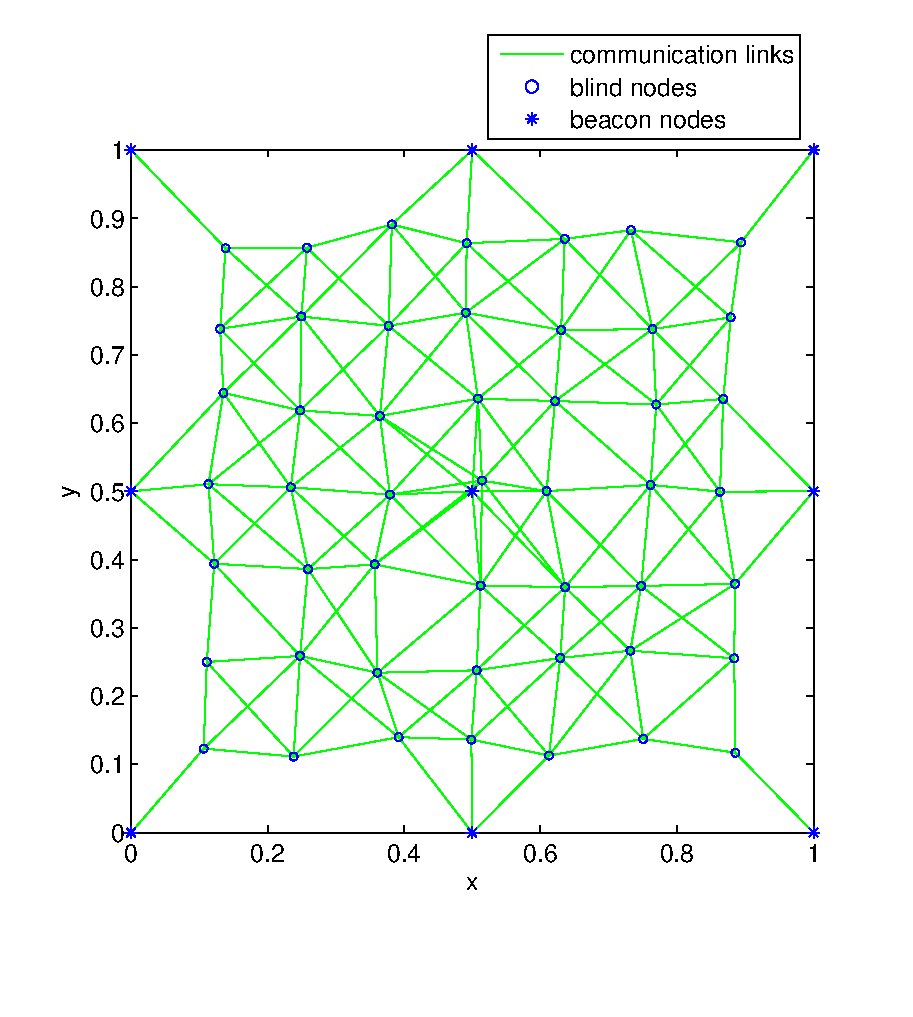
\includegraphics[width=0.6\textwidth]{xy.eps}
\vspace*{-1.3cm}
\caption{True positions of nodes in the WSN and the communication topology in the simulation example in Section \ref{myex}.}
\end{figure}

\begin{figure}[!t]\label{xye}
\centering
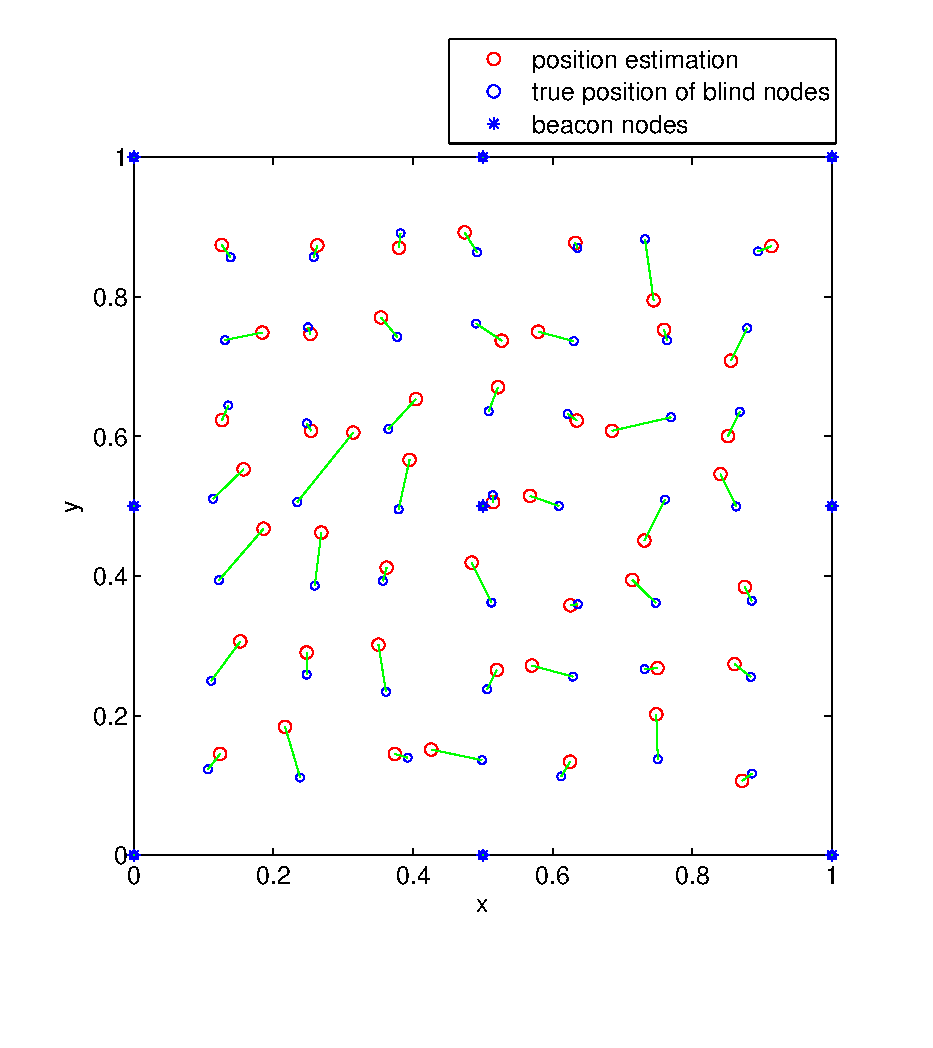
\includegraphics[width=0.6\textwidth]{xye.eps}
\vspace*{-1.3cm}
\caption{Position estimation results in the simulation example in Section \ref{myex}.}
\end{figure}

\begin{figure}[!t]\label{xtrans}
\centering
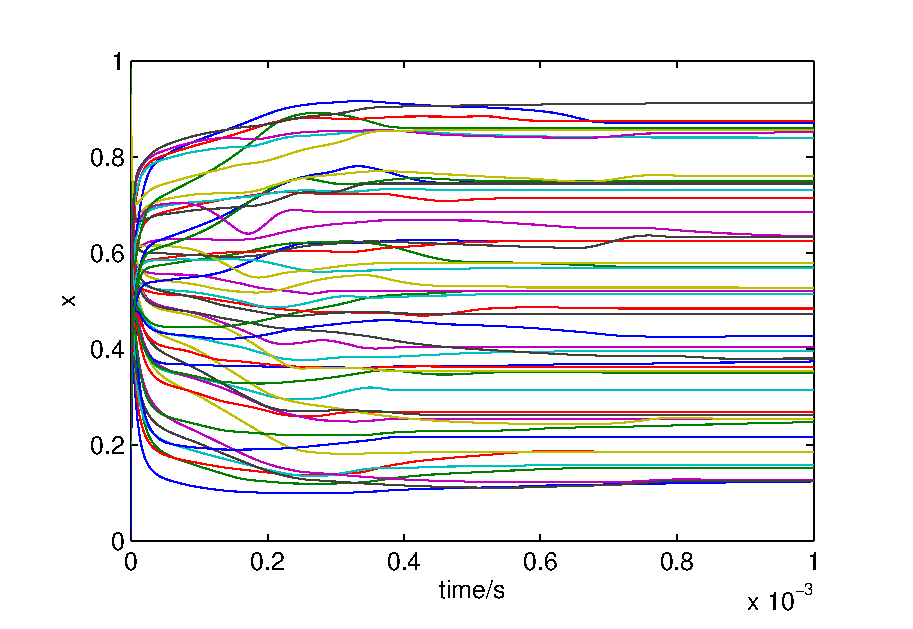
\includegraphics[width=0.6\textwidth]{xtrans.eps}
\caption{Transient of the position estimation in x-direction in the simulation example in Section \ref{myex}.}
\end{figure}

\begin{figure}[!t]\label{ytrans}
\centering
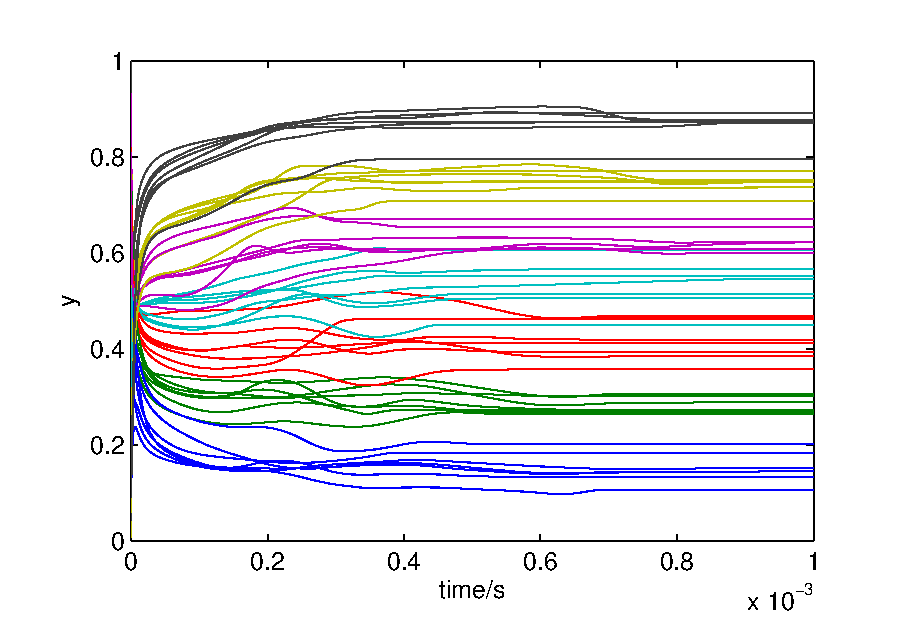
\includegraphics[width=0.6\textwidth]{ytrans.eps}
\caption{Transient of the position estimation in y-direction in the simulation example in Section \ref{myex}.}
\end{figure}

\subsection{Random Placement}\label{hellow}
In this set of experiments, $150$ blind nodes are randomly deployed to a normalized $1\times 1$ square with $9$ beacon nodes locating at $[0, 0]$, $[0.5, 0]$, $[1, 0]$, $[1, 0.5]$, $[1, 1]$, $[0.5, 1]$, $[0, 1]$, $[0, 0.5]$, $[0.5, 0.5]$ as shown in Fig. $6$. The maximum sensor range is set to be $R=0.15$ and the scaling factor $\epsilon=10^5$ for the neural network. Fig. $7$ shows the estimated positions of blind sensor by running the neural network for $10^{-3}$ seconds. The transient of estimated positions in x and y directions are plotted in Fig. $8$ and Fig. $9$, respectively. Fig. $10$ shows the evolution of $\sum_{j\in\mathbb{N}_i, i\in\mathbb{V}} max(\|x_i-x_j\|^2, 0)$ with time, which is an quantitive evaluation of the feasibility of the solution to the WSN localization problem (\ref{wsnm}). The value starts from  $387.1349$ and drops to $0.0106$ at the end of the simulation, which demonstrates the effectiveness of the proposed approach.


\begin{figure}[!t]\label{xy1}
\centering
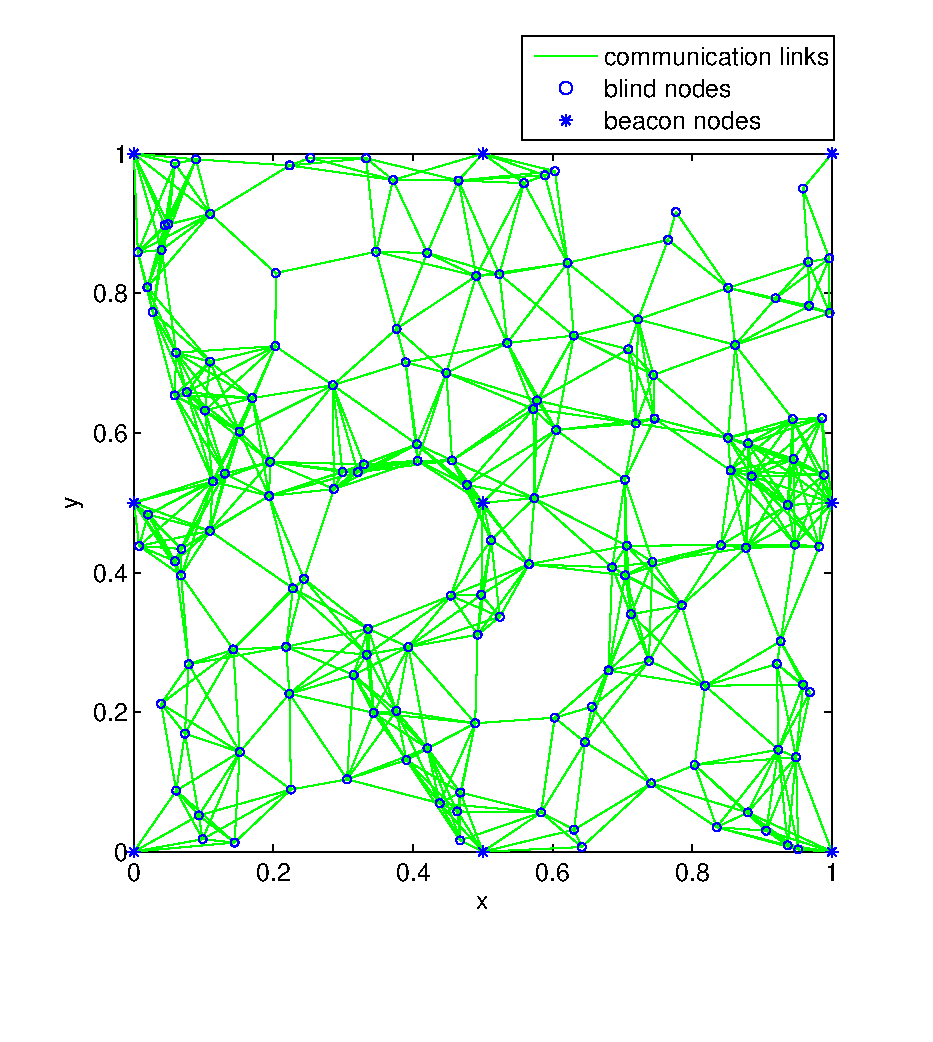
\includegraphics[width=0.6\textwidth]{xy1.eps}
\vspace*{-1.3cm}
\caption{True positions of nodes in the WSN and the communication topology in the simulation example in Section \ref{hellow}.}
\end{figure}

\begin{figure}[!t]\label{xye1}
\centering
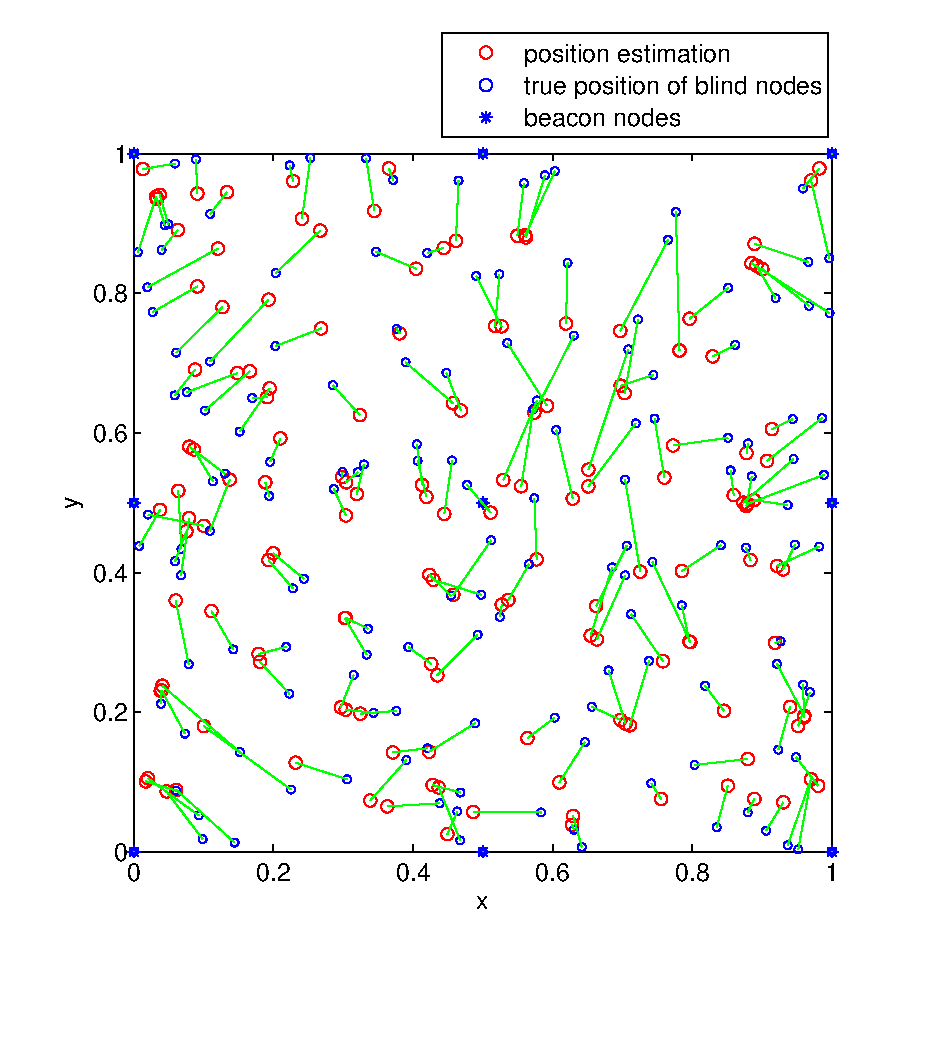
\includegraphics[width=0.6\textwidth]{xye1.eps}
\vspace*{-1.3cm}
\caption{Position estimation results in the simulation example in Section \ref{hellow}.}
\end{figure}

\begin{figure}[!t]\label{xtrans1}
\centering
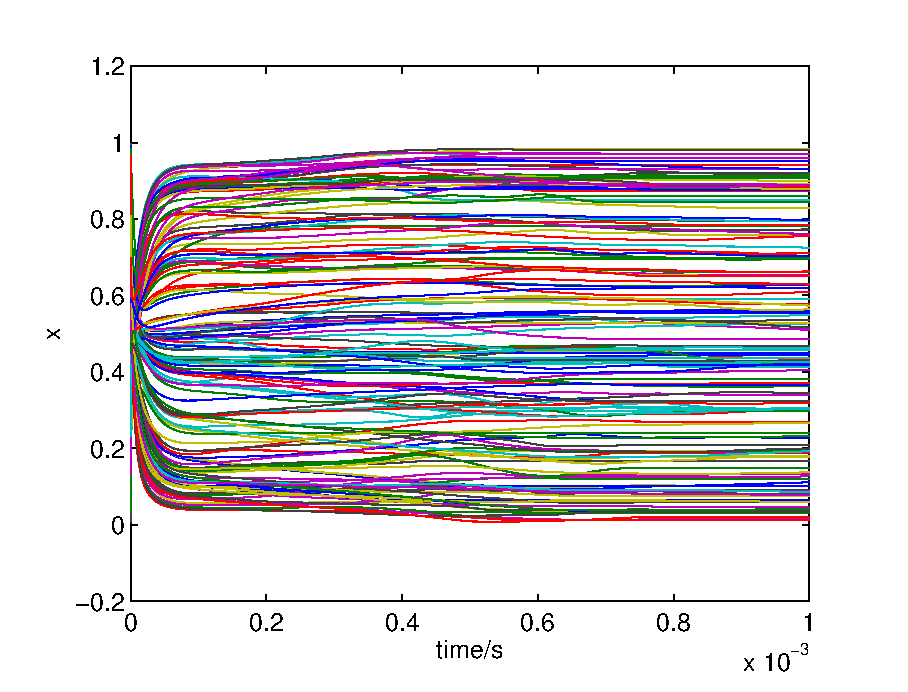
\includegraphics[width=0.6\textwidth]{xtrans1.eps}
\caption{Transient of the position estimation in x-direction in the simulation example in Section \ref{hellow}.}
\end{figure}

\begin{figure}[!t]\label{ytrans1}
\centering
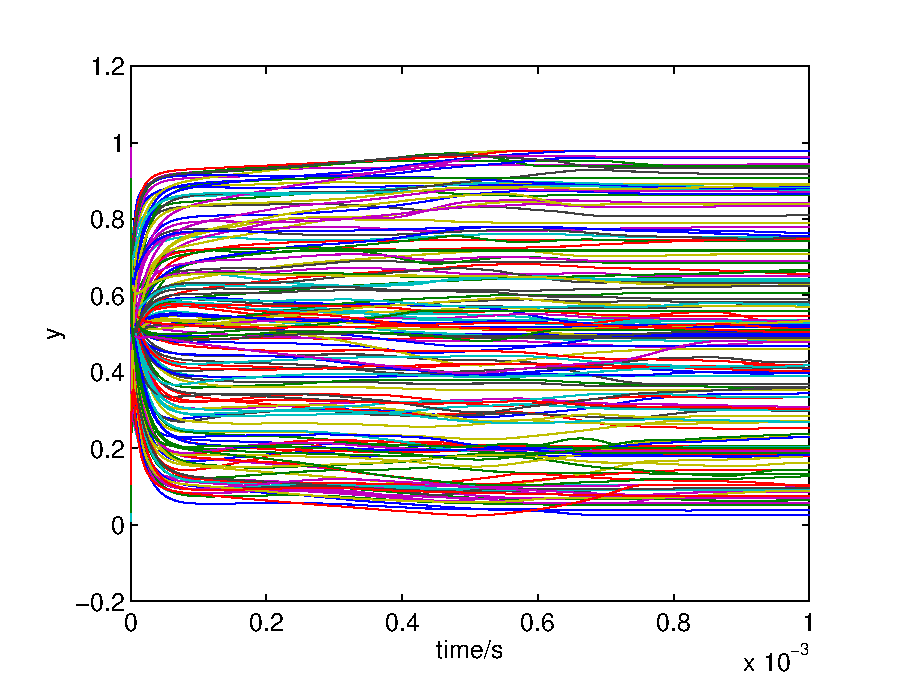
\includegraphics[width=0.6\textwidth]{ytrans1.eps}
\caption{Transient of the position estimation in y-direction in the simulation example in Section \ref{hellow}.}
\end{figure}

\begin{figure}[!t]\label{new}
\centering
\includegraphics[width=0.7\textwidth]{new.eps}
\caption{Time evolution of $\sum_{j\in\mathbb{N}_i, i\in\mathbb{V}} max(\|x_i-x_j\|^2-R^2, 0)$ in Section \ref{hellow}.}
\end{figure}




We use  $E=\sqrt{\sum_{i=1}^n{(x_i-x^r_{i})}^T{(x_i-x^r_{i})}/n}$ with  $x^r_{i}$ denoting the real position of the $i$th blind sensor node, to evaluate the localization accuracy of the proposed method. Table \ref{nnn} shows the localization error and the simulation time averaged by running Monte Carlo simulation for $50$ times. The simulation is performed with the programming language Matlab $7.8$ on a laptop with the Intel (R) Core(TM) 2 Duo CPU at $1.80$ GHz and $2$GB of RAM. Note that the simulation program performs the localization algorithms for all the beacon nodes and all the blind nodes. In real application, the localization algorithm will be run in a distributed manner separately by all nodes. In all simulations, the beacon nodes are evenly deployed in space. As observed in the table, the localization error is around $0.15$ for the case with $9$ beacons. With the increase of beacons, the localization error decreases. For the case with $36$ beacons, the changes of blind node numbers have small influences to the localization error and the value is around $0.6$. As to the PC time (the CPU time in the simulation), it increases with the increase of the number of sensor nodes.  It is worth noting that the theoretical running time of the proposed algorithm is much less than the PC time. This is because, on one hand, the simulation program simulates all nodes on a single computer while the algorithm is expected to run separately on all  sensors in parallel in real application and on the other hand  the neural network implementation in analog circuits can complete the computation when the neural evolution converges. As to the software implementation of the neural network model, the running time can be estimated by the ratio between the PC time listed in the table and the total number of nodes simulated, whose value is still acceptable for real-time processing.




\begin{table}
\centering
\scriptsize
\begin{tabular}{c|c||c|c|c}
\hline
\multicolumn{2}{c||}{Parameters}&\multicolumn{3}{c}{Performances}\\\hline
\tabincell{c}{No. of\\ beacons}& \tabincell{c}{No. of \\ blind sensors} & \tabincell{c}{Average Localization\\  Error}& \tabincell{c}{Average PC \\ time(seconds)} & \tabincell{c}{Theoretical \\ time (seconds)}
\\ \hline
 9 & 110  &0.1756&11.193993&$1.0\times 10^{-4}$\\\hline
 9  & 130 &0.1701&15.187071&$1.0\times 10^{-4}$\\\hline
 9  & 150 &0.1309&20.810211&$1.0\times 10^{-4}$\\\hline
 9 & 170  &0.1549&26.104286&$1.0\times 10^{-4}$\\\hline
 16 & 110 &0.0995&14.219097&$1.0\times 10^{-4}$\\\hline
 16 & 130 &0.0904&17.293275&$1.0\times 10^{-4}$\\\hline
 16 & 150 &0.0912&23.444137&$1.0\times 10^{-4}$\\\hline
 16 & 170 &0.0947&27.156888&$1.0\times 10^{-4}$\\\hline
 25 & 110 &0.0751&15.964024&$1.0\times 10^{-4}$\\\hline
 25 & 130 &0.0700&19.236726&$1.0\times 10^{-4}$\\\hline
 25 & 150 &0.0669&24.460955&$1.0\times 10^{-4}$\\\hline
 25 & 170 &0.0684&31.058264&$1.0\times 10^{-4}$\\\hline
 36 & 110 &0.0672&16.791616&$1.0\times 10^{-4}$\\\hline
 36 & 130 &0.0658&21.397013&$1.0\times 10^{-4}$\\\hline
 36 & 150 &0.0645&26.174775&$1.0\times 10^{-4}$\\\hline
 36 & 170 &0.0619&31.232622&$1.0\times 10^{-4}$\\\hline
\end{tabular}
\caption{Performances under different parameter setups.}\label{nnn}
\end{table}








\section{Conclusions}\label{cons}
In this paper, we define the problem of finding a feasible solution to a class of nonlinear inequalities defined on a graph and propose a recurrent neural network approach to solve this problem. The convergence of the proposed neural network and the feasibility of the solution are proven in theory. This neural network approach is applied to WSN localization in a distributed, routing-free, range-free way and the architecture of the circuit implementation of the neural network for WSN localization is given. Finally, simulations demonstrate efficiency and accuracy of the method.



%\section*{Acknowledgements}
%The authors would like to acknowledge the support by  Guangdong Science Foundation of China under Grant  $S2011010006116$, the National Natural Science Foundation of China under Grant No. $61172165$, and Science and Technology Planning Project of shenzhen city under Grant No. $JC200903180648A$.
%



%\useRomanappendicesfalse
%\appendices
%\section{Proof of Proposition \ref{transformation1}} \label{appA}
%Because of
%\begin{eqnarray}\label{T0constraint1}
%  \mathbf{I}=\mathbf{T}\mathbf{T}^T=\left[
%  \begin{array}{cc}
%    \mathbf{T}_{0}\mathbf{T}_{0}^{T} & \mathbf{T}_{0}\frac{\mathbf{1}}{\sqrt{n}} \\
%    \frac{\mathbf{1}^T}{\sqrt{n}}\mathbf{T}_0^T & 1
%  \end{array}
%  \right]
%\end{eqnarray}
%\begin{eqnarray}\label{T0constraint2}
% \mathbf{I}=\mathbf{T}^T\mathbf{T}=\left[
%  \begin{array}{c}
%    \mathbf{T}_{0}^{T}\mathbf{T}_{0}+\frac{\mathbf{1}\mathbf{1}^T}{n}
%  \end{array}
%  \right]
%\end{eqnarray}
%we have,
%\begin{eqnarray}\label{T0constraintclear1}
%&\mathbf{T}_0\mathbf{1}=\mathbf{0}\nonumber\\
%&\mathbf{T}_0\mathbf{T}_0^T=\mathbf{I}\nonumber\\
%&\mathbf{T}_0^T\mathbf{T}_0=\mathbf{I}-\frac{\mathbf{1}\mathbf{1}^T}{n}
%\end{eqnarray}
%Representing the system (\ref{protocoldisturbance}) by the new
%variable $\mathbf{y}(t)$, we have:
%\begin{eqnarray}
%&\quad&\mathbf{y}(t+1)\nonumber\\
%&=&\mathbf{T}\mathbf{W}\mathbf{T}^T\mathbf{y}(t)-\mathbf{T}\mathbf{L}\mathbf{v}(t)\nonumber\\
%&=&\left[
%  \begin{array}{cc}
%    \mathbf{T}_{0}\mathbf{W}\mathbf{T}_{0}^T & \mathbf{T}_{0}\mathbf{W}\frac{\mathbf{1}}{\sqrt{n}} \\
%    \frac{\mathbf{1}^T}{\sqrt{n}}\mathbf{W}\mathbf{T}_{0}^T & \frac{\mathbf{1}^T}{\sqrt{n}}\mathbf{W}\frac{\mathbf{1}}{\sqrt{n}}
%  \end{array}
%  \right]\mathbf{y}(t)-\left[
%  \begin{array}{c}
%    \mathbf{T}_{0}\mathbf{L}\mathbf{v}(t) \\
%    \frac{\mathbf{1}^T}{\sqrt{n}}\mathbf{L}\mathbf{v}(t)
%  \end{array}
%  \right]\nonumber\\
%&\quad&
%  \end{eqnarray}
%For the connected and balanced graph, $\mathbf{W}$ is a doubly
%stochastic matrix. Therefore,$\mathbf{W}\mathbf{1}=\mathbf{1}$ and
%$\mathbf{1}^T\mathbf{W}=\mathbf{1}^T$. Since
%$\mathbf{L}=\mathbf{I}-\mathbf{W}$, we have
%$\mathbf{1}^T\mathbf{L}=\mathbf{1}^T-\mathbf{1}^T\mathbf{W}=\mathbf{0}$.
%Together with (\ref{T0constraintclear1}), we get
%\begin{eqnarray}
%  \mathbf{y}(t+1)=\left[
%  \begin{array}{cc}
%    \mathbf{T}_{0}\mathbf{W}\mathbf{T}_{0}^T & \mathbf{0} \\
%    \mathbf{0} & 1
%  \end{array}
%  \right]\mathbf{y}(t)-\left[
%  \begin{array}{c}
%    \mathbf{T}_{0}\mathbf{L}\mathbf{v}(t) \\
%    0
%  \end{array}
%  \right]
%\end{eqnarray}
%That is,
%\begin{eqnarray}
%&\mathbf{y}_0(t+1)=\mathbf{T}_{0}\mathbf{W}\mathbf{T}_{0}^T\mathbf{y}_0(t)-\mathbf{T}_{0}\mathbf{L}\mathbf{v}(t)\nonumber\\
%&\mathbf{y}_a(t+1)= \mathbf{y}_a(t)
%\end{eqnarray}
%As to the output $\mathbf{z}(t)$, we can represent it in term of
%$\mathbf{y}_0(t)$:
%\begin{eqnarray}
%\mathbf{z}(t)=&\mathbf{x}(t)-
%\frac{\mathbf{1}\mathbf{1}^T\mathbf{x}(0)}{n}\nonumber\\
%=&\mathbf{x}(t)- \frac{\mathbf{1}\mathbf{1}^T\mathbf{x}(t)}{n}\nonumber\\
%=&\mathbf{T}_0^T\mathbf{T}_0\mathbf{x}(t)\nonumber\\
%=&\mathbf{T}_0^T\mathbf{y}_0(t)
%\end{eqnarray}
%The transformation matrix $\mathbf{T}$ is orthogonal, so the new
%system with $\mathbf{y}$ as the state is equivalent to the
%original one.
%This completes the proof.%end of proof
%
%
%
%
%
%\section{Proof of Lemma \ref{matrixinequality1}} \label{appB}
%
%Define the Lyapunov function as follows:
%\begin{eqnarray}
%V(t)=\mathbf{y}_0^T(t)\mathbf{P}\mathbf{y}_0(t)
%\end{eqnarray}
%where $\mathbf{P}$ is a symmetric positive definite matrix. Denote
%\begin{eqnarray}
%J(t)=\sum_{\tau=0}^{t}\mathbf{z}^T(\tau)\mathbf{z}(\tau)-\gamma^2\mathbf{v}^T(\tau)\mathbf{v}(\tau)
%\end{eqnarray}
%Representing $\mathbf{z}(\tau)$ by $\mathbf{y}_0(\tau)$, we have
%\begin{eqnarray}
%J(t)=\sum_{\tau=0}^{t}\mathbf{y}_0^T(\tau)\mathbf{T}_0\mathbf{T}_0^T\mathbf{y}_0(\tau)-\gamma^2\mathbf{v}^T(\tau)\mathbf{v}(\tau)
%\end{eqnarray}
%Recalling $\mathbf{T}_0\mathbf{T}_0^T=\mathbf{I}$, $J(t)$ is
%simplified to:
%\begin{eqnarray}
%J(t)=\sum_{\tau=0}^{t}\mathbf{y}_0^T(\tau)\mathbf{y}_0(\tau)-\gamma^2\mathbf{v}^T(\tau)\mathbf{v}(\tau)
%\end{eqnarray}
%Note that
%\begin{align}\label{vtv0}
%\quad & V(t+1)-V(0)\nonumber\\
%=&\sum_{\tau=0}^{t}V(\tau+1)-V(\tau)\nonumber\\
%=&\sum_{\tau=0}^{t}\mathbf{y}_0^T(\tau+1)\mathbf{P}\mathbf{y}_0(\tau+1)-\mathbf{y}_0^T(\tau)\mathbf{P}\mathbf{y}_0(\tau)
%\end{align}
%Substituting the expression of $\mathbf{y}_0(\tau+1)$ into
%equation (\ref{vtv0}), we get
%\begin{align}
%V(t+1)-V(0)=&\sum_{\tau=0}^{t}\bigg(\mathbf{y}_0^T(\tau)(\mathbf{T}_0\mathbf{W}^T\mathbf{T}_0^T\mathbf{P}\mathbf{T}_0\mathbf{W}\mathbf{T}_0^T\nonumber\\
%&-\mathbf{P})\mathbf{y}_0(\tau)+\mathbf{v}^T(\tau)\mathbf{L}^T\mathbf{T}_0^T\mathbf{P}\mathbf{T}_0\mathbf{L}\mathbf{v}(\tau)\nonumber\\
%&-\mathbf{y}_0^T(\tau)\mathbf{T}_0\mathbf{W}^T\mathbf{T}_0^T\mathbf{P}\mathbf{T}_0\mathbf{L}\mathbf{v}(\tau)\nonumber\\
%&-\mathbf{v}^T(\tau)\mathbf{L}^T\mathbf{T}_0^T\mathbf{P}\mathbf{T}_0\mathbf{W}\mathbf{T}_0^T\mathbf{y}_0(\tau)\bigg)
%\end{align}
%Therefore, we obtain
%\begin{align}
%J(t)+V(t)-V(0)=&\sum_{\tau=0}^{t}\bigg(\mathbf{y}_0^T(\tau)(\mathbf{T}_0\mathbf{W}^T\mathbf{T}_0^T\mathbf{P}\mathbf{T}_0\mathbf{W}\mathbf{T}_0^T\nonumber\\
%&-\mathbf{P}+\mathbf{I})\mathbf{y}_0(\tau)+\mathbf{v}^T(\tau)(-\gamma^2\mathbf{I}\nonumber\\
%&+\mathbf{L}^T\mathbf{T}_0^T\mathbf{P}\mathbf{T}_0\mathbf{L})\mathbf{v}(\tau)\nonumber\\
%&-\mathbf{y}_0^T(\tau)\mathbf{T}_0\mathbf{W}^T\mathbf{T}_0^T\mathbf{P}\mathbf{T}_0\mathbf{L}\mathbf{v}(\tau)\nonumber\\
%&-\mathbf{v}^T(\tau)\mathbf{L}^T\mathbf{T}_0^T\mathbf{P}\mathbf{T}_0\mathbf{W}\mathbf{T}_0^T\mathbf{y}_0(\tau)\bigg)
%\end{align}
%This can be written in a quadratic form,
%\begin{align}
%J(t)+V(t)-V(0)=\sum_{\tau=0}^{t}\bigg(\left[ \mathbf{y}_0^T(\tau),
%\mathbf{v}^T(\tau) \right]\nonumber
%\end{align}
%$\cdot\left[
%  \begin{array}{cc}
%   \mathbf{I}+\mathbf{T}_0\mathbf{W}^T\mathbf{T}_0^T\mathbf{P}\mathbf{T}_0\mathbf{W}\mathbf{T}_0^T-\mathbf{P} & -\mathbf{T}_0\mathbf{W}^T\mathbf{T}_0^T\mathbf{P}\mathbf{T}_0\mathbf{L}\\
%-\mathbf{L}^T\mathbf{T}_0^T\mathbf{P}\mathbf{T}_0\mathbf{W}\mathbf{T}_0^T
%& -\gamma^2\mathbf{I}+\mathbf{L}^T\mathbf{T}_0^T\mathbf{P}
%\mathbf{T}_0\mathbf{L}
%  \end{array}
%\right]$
%
%$\cdot\left[
%\begin{array}{c}
%\mathbf{y}_0(\tau)\\
% \mathbf{v}(\tau)
% \end{array}
% \right]\bigg)$
%\begin{align}
%\end{align}
%Since
%\begin{align}
%&\left[
%  \begin{array}{cc}
%   \mathbf{I}+\mathbf{T}_0\mathbf{W}^T\mathbf{T}_0^T\mathbf{P}\mathbf{T}_0\mathbf{W}\mathbf{T}_0^T-\mathbf{P} & -\mathbf{T}_0\mathbf{W}^T\mathbf{T}_0^T\mathbf{P}\mathbf{T}_0\mathbf{L}\\
%-\mathbf{L}^T\mathbf{T}_0^T\mathbf{P}\mathbf{T}_0\mathbf{W}\mathbf{T}_0^T
%& -\gamma^2\mathbf{I}+\mathbf{L}^T\mathbf{T}_0^T\mathbf{P}
%\mathbf{T}_0\mathbf{L}
%  \end{array}
%\right]\nonumber\\
%&<0
%\end{align}
%we have
%\begin{align}
%& \quad J(t)<-V(t)+V(0)\nonumber\\
%&\Rightarrow J(t)<V(0)\nonumber\\
%&\Rightarrow
%\sup_{t>0}\sum_{\tau=0}^{t}\mathbf{z}^T(\tau)\mathbf{z}(\tau)-\gamma^2\mathbf{v}^T(\tau)\mathbf{v}(\tau)<V(0)
%\end{align}
%Choosing a constant not less than $V(0)$ leads to the conclusion. This concludes the proof of Lemma \ref{matrixinequality1}. % end of proof
%
%
%
%
%\section{Proof of Theorem \ref{lmiexpression1}} \label{appC}
%
%The proof that system  (\ref{protocoldisturbanceandz}) has a
%bounded consensus error follows the argument in Remark
%\ref{remarkbibo}. Now we prove the rest part of Theorem
%\ref{lmiexpression1}. Since
%$\text{diag}([\mathbf{I},\mathbf{Q}^{-1},\mathbf{I},\mathbf{I}])$
%has full rank, we have
%\begin{eqnarray}
%&\left[
%  \begin{array}{cccc}
%   -\mathbf{Q} & \mathbf{S} & -\mathbf{T}_0\mathbf{L} & \mathbf{0}\\
%   \mathbf{S}^T & -\mathbf{Q} & \mathbf{0} & \mathbf{Q}\mathbf{T}_0\\
%   -\mathbf{L}^T\mathbf{T}_0^T & \mathbf{0} & -\gamma^2\mathbf{I} & \mathbf{0}\\
%   \mathbf{0} & \mathbf{T}_0^T\mathbf{Q} & \mathbf{0} &
%   -\mathbf{I}
%  \end{array}
%\right]<0 \nonumber\\
%\Leftrightarrow &
%\text{diag}([\mathbf{I}\,\mathbf{Q}^{-1}\,\mathbf{I}\,\mathbf{I}])
% \left[
%  \begin{array}{cccc}
%   -\mathbf{Q} & \mathbf{S} & -\mathbf{T}_0\mathbf{L} & \mathbf{0}\\
%   \mathbf{S}^T & -\mathbf{Q} & \mathbf{0} & \mathbf{Q}\mathbf{T}_0\\
%   -\mathbf{L}^T\mathbf{T}_0^T & \mathbf{0} & -\gamma^2\mathbf{I} & \mathbf{0}\\
%   \mathbf{0} & \mathbf{T}_0^T\mathbf{Q} & \mathbf{0} & -\mathbf{I}
%  \end{array}
%\right]\nonumber\\
%&\cdot\text{diag}([\mathbf{I}\,\mathbf{Q}^{-1}\,\mathbf{I}\,\mathbf{I}])<0\nonumber\\
%\Leftrightarrow &
% \left[
% \begin{array}{*{20}c}
%   -\mathbf{Q} & \mathbf{S}\mathbf{Q}^{-1} & -\mathbf{T}_0\mathbf{L} & \vline & \mathbf{0}\\
%   \mathbf{Q}^{-1}\mathbf{S}^T & -\mathbf{Q}^{-1} & \mathbf{0} & \vline & \mathbf{T}_0\\
%   -\mathbf{L}^T\mathbf{T}_0^T & \mathbf{0} & -\gamma^2\mathbf{I} & \vline & \mathbf{0}\\
%   \hline
%   \mathbf{0} & \mathbf{T}_0^T & \mathbf{0} & \vline & -\mathbf{I}
%  \end{array}
%\right]<0
%\end{eqnarray}
%Using the Schur complement, we get the following equivalent
%inequality:
%\begin{align}
%&\left[
% \begin{array}{ccc}
%   -\mathbf{Q} & \mathbf{S}\mathbf{Q}^{-1} & -\mathbf{T}_0\mathbf{L} \\
%   \mathbf{Q}^{-1}\mathbf{S}^T & -\mathbf{Q}^{-1} & \mathbf{0} \\
%   -\mathbf{L}^T\mathbf{T}_0^T & \mathbf{0} & -\gamma^2\mathbf{I}
%\end{array}
%\right]-
% \left[
% \begin{array}{c}
%   \mathbf{0} \\
%   \mathbf{T}_0 \\
%   \mathbf{0}
%\end{array}
%\right](-\mathbf{I})^{-1}\nonumber\\
%&\cdot \left[
% \begin{array}{ccc}
%   \mathbf{0}&
%   \mathbf{T}_0^T&
%   \mathbf{0}
%\end{array}
%\right] <0\nonumber\\
%&\Leftrightarrow
% \left[
% \begin{array}{*{20}c}
%   -\mathbf{Q} & \vline & \mathbf{S}\mathbf{Q}^{-1} & -\mathbf{T}_0\mathbf{L} \\
%   \hline
%   \mathbf{Q}^{-1}\mathbf{S}^T & \vline & -\mathbf{Q}^{-1}+\mathbf{T}_0\mathbf{T}_0^T & \mathbf{0} \\
%   -\mathbf{L}^T\mathbf{T}_0^T & \vline & \mathbf{0} &
%   -\gamma^2\mathbf{I}
%\end{array}
%\right]<0
%\end{align}
%Using the Schur complement to this inequality, we equivalently
%get:
%\begin{align}
%&\left[
% \begin{array}{*{20}c}
%   -\mathbf{Q}^{-1}+\mathbf{T}_0\mathbf{T}_0^T & \mathbf{0} \\
%   \mathbf{0} & -\gamma^2\mathbf{I}
%\end{array}
%\right] - \left[
% \begin{array}{c}
% \mathbf{Q}^{-1}\mathbf{S}^T\\
%  -\mathbf{L}^T\mathbf{T}_0^T
%\end{array}
%\right](-\mathbf{Q})^{-1}\nonumber\\
%&\cdot \left[
% \begin{array}{cc}
% \mathbf{S}\mathbf{Q}^{-1}&
%  -\mathbf{T}_0\mathbf{L}
%\end{array}
%\right]<0
%\end{align}
%Recalling $\mathbf{T}_0\mathbf{T}_0^T=\mathbf{I}$,
%$\mathbf{S}=\mathbf{T}_0\mathbf{W}\mathbf{T}_0^T\mathbf{Q}$,
%defining $\mathbf{P}=\mathbf{Q}^{-1}$ and then substituting them
%into the expression, we can finally get the
%expression of (\ref{lmi21}), which concludes the proof.% end of proof
%
%
%
%
%\section{Proof of Theorem \ref{convergetheorem}} \label{appD}
%
%According to equation (\ref{newvariableprotocol}), we have
%\begin{align}
%\mathbf{y}_0(t+1)\mathbf{y}_0^T(t+1)=&\mathbf{T}_0\mathbf{W}\mathbf{T}_0^T\mathbf{y}_0(t)\mathbf{y}_0^T(t)\mathbf{T}_0\mathbf{W}^T\mathbf{T}_0^T\nonumber\\
%&+\mathbf{T}_0\mathbf{L}\mathbf{v}(t)\mathbf{v}^T(t)\mathbf{L}^T\mathbf{T}_0^T\nonumber\\
%&-\mathbf{T}_0\mathbf{W}\mathbf{T}_0^T\mathbf{y}_0(t)\mathbf{v}^T(t)\mathbf{L}^T\mathbf{T}_0^T\nonumber\\
%&-\mathbf{T}_0\mathbf{L}\mathbf{v}(t)\mathbf{y}_0^T(t)\mathbf{T}_0\mathbf{W}^T\mathbf{T}_0^T
%\end{align}
%Calculating the expected value on both sides, we get
%\begin{align}
%\quad & E(\mathbf{y}_0(t+1)\mathbf{y}_0^T(t+1))\nonumber\\
%=&\mathbf{T}_0\mathbf{W}\mathbf{T}_0^TE(\mathbf{y}_0(t)\mathbf{y}_0^T(t))\mathbf{T}_0\mathbf{W}^T\mathbf{T}_0^T\nonumber\\
%&+\mathbf{T}_0\mathbf{L}E(\mathbf{v}(t)\mathbf{v}^T(t))\mathbf{L}^T\mathbf{T}_0^T
%\end{align}
%Defining a new variable
%$\mathbf{\Sigma}_{y0}(t)=E(\mathbf{y}_0(t)\mathbf{y}_0^T(t))$ and
%noting that $E(\mathbf{v}(t)\mathbf{v}^T(t))=\mathbf{\Sigma}_v$,
%which is a constant matrix, we have,
%\begin{align}
%\mathbf{\Sigma}_{y0}(t+1)=\mathbf{T}_0\mathbf{W}\mathbf{T}_0^T\mathbf{\Sigma}_{y0}(t)\mathbf{T}_0\mathbf{W}^T\mathbf{T}_0^T+\mathbf{T}_0\mathbf{L}\mathbf{\Sigma}_v\mathbf{L}^T\mathbf{T}_0^T
%\end{align}
%Use the Kronecker product to write $\mathbf{\Sigma}_{y0}(t+1)$ in
%a vector form,
%\begin{align}
%\text{vec}(\mathbf{\Sigma}_{y0}(t+1))=&((\mathbf{T}_0\mathbf{W}\mathbf{T}_0^T)\otimes(\mathbf{T}_0\mathbf{W}\mathbf{T}_0^T))\text{vec}(\mathbf{\Sigma}_{y0}(t))\nonumber\\
%&+((\mathbf{T}_0\mathbf{L})\otimes(\mathbf{T}_0\mathbf{L}))\text{vec}(\mathbf{\Sigma}_v)
%\end{align}
%This is a linear time invariant system and therefore we can study
%its system matrix for the convergence. The eigenvalues of
%$(\mathbf{T}_0\mathbf{W}\mathbf{T}_0^T)\otimes(\mathbf{T}_0\mathbf{W}\mathbf{T}_0^T)$
%are represented by the eigenvalues of
%$\mathbf{T}_0\mathbf{W}\mathbf{T}_0^T$ as $\lambda_i\lambda_j$ for
%$i=1, 2, ..., n, j=1, 2, ..., n$, where $\lambda_i$ is the $i$-th
%eigenvalue of $\mathbf{T}_0\mathbf{W}\mathbf{T}_0^T$. In addition,
%the magnitude of the stochastic matrix
%$\mathbf{T}_0\mathbf{W}\mathbf{T}_0^T$'s eigenvalue $\lambda_i$
%satisfies $|\lambda_i|<1$ as argued before. Therefore, we conclude
%that all eigenvalues of
%$(\mathbf{T}_0\mathbf{W}\mathbf{T}_0^T)\otimes(\mathbf{T}_0\mathbf{W}\mathbf{T}_0^T)$
%have magnitude less than 1. That is,
% $|\text{eig}((\mathbf{T}_0\mathbf{W}\mathbf{T}_0^T)\otimes(\mathbf{T}_0\mathbf{W}\mathbf{T}_0^T))|<1$.
%
%Hence, $\mathbf{\Sigma}_{y0}(t)$ converges eventually. Denoting
%$\mathbf{\Sigma}_{y0}$ as its steady state value, we can calculate
%it easily by solving the steady state linear equation. After
%calculation, we have,
%\begin{align}
%\text{vec}(\mathbf{\Sigma}_{y0})=&(\mathbf{I}-(\mathbf{T}_0\mathbf{W}\mathbf{T}_0^T)\otimes(\mathbf{T}_0\mathbf{W}\mathbf{T}_0^T))^{-1}((\mathbf{T}_0\mathbf{L})\nonumber\\
%&\otimes(\mathbf{T}_0\mathbf{L}))\text{vec}(\mathbf{\Sigma}_v)
%\end{align}
%Thus,
%\begin{align}
%\text{vec}(\mathbf{\Sigma}_{z})=&(\mathbf{I}\otimes
%\mathbf{T}_0^T)\text{vec}(\mathbf{\Sigma}_{y0})\nonumber\\
%=&(\mathbf{I}\otimes
%\mathbf{T}_0^T)(\mathbf{I}-(\mathbf{T}_0\mathbf{W}\mathbf{T}_0^T)\nonumber\\
%&\otimes(\mathbf{T}_0\mathbf{W}\mathbf{T}_0^T))^{-1}((\mathbf{T}_0\mathbf{L})\otimes(\mathbf{T}_0\mathbf{L}))\text{vec}(\mathbf{\Sigma}_v)
%\end{align}
%This concludes the proof of Theorem \ref{convergetheorem}.
%%end of proof
%
%
%
%\section{Proof of Theorem \ref{meansquareerror}} \label{appE}
%Since
%$\mathbf{z}^T(t)\mathbf{z}(t)=\text{trace}(\mathbf{z}(t)\mathbf{z}^T(t))$
%and $E(\mathbf{z}(t)\mathbf{z}^T(t))$ converges (Theorem
%\ref{convergetheorem}), we conclude $\lim_{t \to
%\infty}E(\frac{\mathbf{z}^T(t)\mathbf{z}(t)}{n})$ exists.
%
%According to the performance index (\ref{l2gain}), we have for all
%$t>0$,
%\begin{align}
%\sum_{\tau=0}^{t}\mathbf{z}^T(\tau)\mathbf{z}(\tau)-\gamma^2\mathbf{v}^T(\tau)\mathbf{v}(\tau)<\text{constant}
%\end{align}
%Calculating expected value on both sides and rewriting the
%expression, we get,
%\begin{align}\label{inequ}
%\sum_{\tau=0}^{t}E(\mathbf{z}^T(\tau)\mathbf{z}(\tau))<&t\gamma^2\text{trace}(E(\mathbf{v}(\tau)\mathbf{v}^T(\tau)))\nonumber\\
%&+\text{constant}
%\end{align}
%For the stochastic quantization, the covariance matrix of
%$\mathbf{v}$ is $\sigma^2\mathbf{I}$. Thus we have
%$\text{trace}(E(\mathbf{v}(\tau)\mathbf{v}^T(\tau)))=n\sigma^2$.
%Substituting this expression into inequality (\ref{inequ}),
%dividing both side of the inequality with $t$ and then calculating
%the limit as $t$ goes to infinity, we have,
%\begin{equation}
%\lim_{t \to
%\infty}E(\frac{\mathbf{z}^T(t)\mathbf{z}(t)}{n})<\gamma^2\sigma^2+\lim_{t
%\to \infty}\frac{\text{constant}}{t}
%\end{equation}
%Since $\lim_{t \to \infty}\frac{\text{constant}}{t}=0$, we get the
%inequality
%(\ref{probilisticconclusion}). This concludes the proof of Theorem \ref{meansquareerror}.%end of proof
%
%
%\section{Proof of Convexity of (\ref{noname9})} \label{appF}
%First, we express
%$\mathbf{W}=\mathbf{I}-\sum_{k=1}^{m}{\omega_k\mathbf{a}_k\mathbf{a}_k^T}$
%with $\mathbf{a}_k$ denoting the $k$th column of the incidence
%matrix of the graph, $\omega_k$ denoting the weight of the $k$th
%edge and $m$ denoting the total amount of edges (see
%\cite{Lin004,Xiao2007} for more detail). In this way, the first
%three constraints in (\ref{noname2}) are satisfied automatically.
%The forth constraint in (\ref{noname2}) can be equivalently
%expressed as the following two LMIs:
%\begin{eqnarray}\label{noname4}
%-\mathbf{I}-\frac{\mathbf{1}\mathbf{1}^T}{n}+\mathbf{W}<0\nonumber\\
%-\mathbf{I}+\frac{\mathbf{1}\mathbf{1}^T}{n}-\mathbf{W}<0
%\end{eqnarray}
%Next, we simplify the expression of $\delta_{ss}$.
%\begin{equation}\label{noname1}
%\mathbf{\Sigma}_z(t+1)=(\mathbf{W}-\frac{\mathbf{1}\mathbf{1}^T}{n})\mathbf{\Sigma}_z(t)(\mathbf{W}-\frac{\mathbf{1}\mathbf{1}^T}{n})+(\mathbf{I}-\mathbf{W})^2\sigma^2
%\end{equation}
%where $\sigma^2$ is the quantization error variance of each node.
%Calculating limits on both sides, we get
%\begin{eqnarray}\label{noname6}
%\mathbf{\Sigma}_{ss}=\sum_{t=0}^{\infty}{(\mathbf{W}-\frac{\mathbf{1}\mathbf{1}^T}{n})^t(\mathbf{I}-\mathbf{W})^2(\mathbf{W}-\frac{\mathbf{1}\mathbf{1}^T}{n})^t\sigma^2}
%\end{eqnarray}
%Since $\sigma^2$ appears to be a coefficient to the expression of
%$\mathbf{\Sigma}_{ss}$ and therefore a coefficient to
%$\delta_{ss}(\mathbf{W})$, we can set $\sigma=1$ without changing
%the optimality. Then, we get
%\begin{eqnarray}\label{noname66}
%&\mathbf{\Sigma}_{ss}\nonumber\\
%=&\sum_{t=0}^{\infty}{(\mathbf{W}-\frac{\mathbf{1}\mathbf{1}^T}{n})^t(\mathbf{I}-\mathbf{W}+\frac{\mathbf{1}\mathbf{1}^T}{n})^2(\mathbf{W}-\frac{\mathbf{1}\mathbf{1}^T}{n})^t\sigma^2}\nonumber\\
%=&(\mathbf{I}+(\mathbf{W}-\frac{\mathbf{1}\mathbf{1}^T}{n})^2-2(\mathbf{W}-\frac{\mathbf{1}\mathbf{1}^T}{n}))\sum_{t=0}^{\infty}{(\mathbf{W}-\frac{\mathbf{1}\mathbf{1}^T}{n})^{2t}}\nonumber\\
%=&(\mathbf{I}+(\mathbf{W}-\frac{\mathbf{1}\mathbf{1}^T}{n})^2-2(\mathbf{W}-\frac{\mathbf{1}\mathbf{1}^T}{n}))(\mathbf{I}-\mathbf{W}^2+\frac{\mathbf{1}\mathbf{1}^T}{n})^{-1}\nonumber\\
%\end{eqnarray}
%The expression can be further simplified via trivial operations
%into the following:
%\begin{eqnarray}\label{noname7}
%\mathbf{\Sigma}_{ss}=2(\mathbf{I}-\mathbf{W}+\frac{\mathbf{1}\mathbf{1}^T}{n})(\mathbf{I}-\mathbf{W}^2+\frac{\mathbf{1}\mathbf{1}^T}{n})^{-1}-\mathbf{I}
%\end{eqnarray}
%With the identity
%$(\mathbf{I}-\mathbf{W}^2+\frac{\mathbf{1}\mathbf{1}^T}{n})^{-1}=\frac{1}{2}(\mathbf{I}+\mathbf{W}-\frac{\mathbf{1}\mathbf{1}^T}{n})^{-1}+\frac{1}{2}(\mathbf{I}-\mathbf{W}+\frac{\mathbf{1}\mathbf{1}^T}{n})^{-1}$,
%we get
%\begin{eqnarray}\label{noname8}
%&\mathbf{\Sigma}_{ss}\nonumber\\
%=&(\mathbf{I}-\mathbf{W}+\frac{\mathbf{1}\mathbf{1}^T}{n})(\mathbf{I}+\mathbf{W}-\frac{\mathbf{1}\mathbf{1}^T}{n})^{-1}\nonumber\\
%=&2(\mathbf{I}+\mathbf{W}-\frac{\mathbf{1}\mathbf{1}^T}{n})^{-1}-\mathbf{I}
%\end{eqnarray}
%With this, we get
%\begin{eqnarray}\label{noname88}
%\delta_{ss}(\mathbf{W})
%=\frac{2}{n}\text{trace}(\mathbf{I}+\mathbf{W}-\frac{\mathbf{1}\mathbf{1}^T}{n})^{-1}-1
%\end{eqnarray}
%Therefore, the problem can be re-stated  as shown in
%(\ref{noname9}). The problem (\ref{noname9}) is a convex problem
%due to the convexity of its constraints and the fact that the
%inverse of a positive definite convex function is still a convex
%function \cite{Xiao2007}. This concludes the proof.



\bibliographystyle{unsrt}   % Include this if you use bibtex
\bibliography{main111}





\end{document}
